\documentclass{beamer}
% \documentclass[handout]{beamer}
\usepackage{natbib}
% no section heading
\renewcommand{\bibsection}{}
\usepackage{amsmath,amsfonts,amsthm,amssymb,euscript,mathrsfs,url,stmaryrd,bbm}
% \usepackage{psfrag}
\usepackage{subfigure}
\usepackage{tikz}

% \usepackage{ragged2e}

\usepackage{color}
\usepackage{import}

% \usepackage{pdfsync}

\usepackage[absolute,overlay]{textpos}

\usepackage[utf8]{inputenc}

% should get rid of superfluous equation labels
\usepackage{mathtools}
\mathtoolsset{showonlyrefs}

\usepackage{multicol}
\usepackage{multirow}
\usepackage{colortbl}
\usepackage{booktabs}

\usepackage[export]{adjustbox}% http://ctan.org/pkg/adjustbox


% theme
\usetheme{Singapore}
\useinnertheme{rounded}
\usecolortheme{rose}
% \usetheme{Warsaw}




%farbversuche
%sieht sehr gut aus aber erstmal nicht
\definecolor{grey}{RGB}{0,0,0}
%aber wir machen erstmal was anderes
\definecolor{darkgreen}{RGB}{90,160,70}
\definecolor{darkred}{RGB}{160,70,70}
\definecolor{brickred}{RGB}{220,55,75}
% \definecolor{yellow}{RGB}{255,255,0}
\definecolor{turquoise}{RGB}{0,255,255}
% \definecolor{grey}{RGB}{0,255,255}
\definecolor{maroon}{RGB}{128,0,0}
\definecolor{purple}{RGB}{155,0,255}



%farbe als structure setzen
\setbeamercolor{structure}{fg=purple!25!black}
% \setbeamercolor{structure}{fg=white!72!black}
%\setbeamercolor{structure}{fg=white!50!green!60!black}


%versuch die textfarbe zu setzen
% \setbeamercolor{normal text}{fg=blue!30!black}
%\setbeamercolor{normal text}{fg=blue}

% cover up
\setbeamercovered{transparent}

% make it work on matthias' laptop
% \setbeamertemplate{blocks}[default]


% macros
\renewcommand{\P}{\mathbb{P}}
\newcommand{\E}{\mathbb{E}}
\newcommand{\V}{\mathbb{V}}
% \newcommand{\N}{\ensuremath{\mathbb{N}}}
\newcommand{\R}{\ensuremath{\mathbb{R}}}
\newcommand{\1}{\ensuremath{\mathbf{1}}}
% \input{macros.tex}

\def\bfmath#1{\mathchoice
        {\mbox{\boldmath$#1$}}%
        {\mbox{\boldmath$#1$}}%
        {\mbox{\boldmath$\scriptstyle#1$}}%
        {\mbox{\boldmath$\scriptscriptstyle#1$}}}%

\def\bfa{\bfmath{a}}
\def\bfb{\bfmath{b}}

\newlength{\nodedist}


\setbeamercolor*{title}{use=structure,fg=white,bg=structure.fg,}
\setbeamertemplate{title page}[default][colsep=-4bp,rounded=true,shadow=true]

%we need this cause sometimes we flip it
\def\defaultbeameritem{ball}
\setbeamertemplate{itemize items}[\defaultbeameritem]


% fancy footline
\setbeamertemplate{footline}
{
\begin{tikzpicture}(0,0)
% % \hbox{%
% \begin{picture}(0,0)
% \tikz\draw[draw=none,top color=white,bottom color=grey!20!white] (0,0) rectangle (\paperwidth,0.25);
\draw[draw=none,top color=white,bottom color=structure.fg!20!white] (0,0) rectangle (\paperwidth,0.25);
\node at (\paperwidth-5,.15) {\insertframenumber};
% \end{picture}
\end{tikzpicture}
% % }%
}
%suppress navigation symbols
\setbeamertemplate{navigation symbols}{}
% % no footline
% \setbeamertemplate{footline}{}
% \setbeamertemplate{footline}[frame number]


% relevant stuff
\title{Overview of mathematical and statistical necessities for population genomics}
% \title{Inferring selection from temporal allele frequency data}
% \author{Matthias Steinrücken\\[2ex]{\footnotesize joint work with}\\{\small Adam Fine and Xiaoheng Cheng}}
\author{Matthias Steinrücken}
% \author{Empirical Population Genomics -- Week 9}
% \institute{Department of Ecology and Evolution, University of Chicago\\ Department of Human Genetics, University of Chicago\\ NITMB} 
% \institute{Department of Ecology and Evolution, University of Chicago\\ Department of Human Genetics, University of Chicago} 
\date{June 8th, 2026}
% \date{}

% \def\newblock{\hskip .11em plus .33em minus .07em}
% \renewcommand{\raggedright}{\leftskip=0pt \rightskip=0pt plus 0cm} 
% \renewcommand{\insertnavigation}[1]{\insertsectionnavigationhorizontal{#1}{}{}}



\begin{document}
%
% \logo{\begin{minipage}[!b]{2cm}\includegraphics[width=1.5cm]{graphics/uc_seal}\end{minipage}
%   \hspace{6cm} \begin{minipage}[!b]{2cm} \includegraphics[width=1.5cm]{graphics/dfg} \end{minipage}
%  \begin{minipage}[!b]{2cm} \includegraphics[width=2cm]{graphics/NIH_logo.png} \end{minipage}}
%
% \logo{\begin{minipage}[!b]{2.5cm}\includegraphics[width=2cm]{graphics/UMassAmherstSeal.png}\\\phantom{menace}\vspace{.2cm}\end{minipage}}
\logo{\begin{minipage}[!b]{2cm}
\includegraphics[width=1.5cm]{graphics/university.seal.rgb.maroon.png}\\\phantom{a}\\\phantom{b}\end{minipage}}
% \logo{}
%
%
%
%%%%%%%%%%%%%%%%%%%%%%%%%%%%%%%%%%%%%%%%%%%%%%%%%%%%%%%%%%%%%%%%%%%%%%%%%%%%%%%%%%%%%%
\begin{frame}
	\titlepage 
	% \addtocounter{framenumber}{-1}
\end{frame}
\logo{}
%%%%%%%%%%%%%%%%%%%%%%%%%%%%%%%%%%%%%%%%%%%%%%%%%%%%%%%%%%%%%%%%%%%%%%%%%%%%%%%%%%%%%%
%
%
%
%%%%%%%%%%%%%%%%%%%%%%%%%%%%%%%%%%%%%%%%%%%%%%%%%%%%%%%%%%%%%%%%%%%%%%%%%%%%%%%%%%%%%%
\begin{frame}{Population genomics}
    \begin{block}{}
        Understand genetic processes that shape genomic variation observed in populations.
    \end{block}
    \begin{enumerate}
        \item Develop computational/mathematical models of these population genetic processes.
        \begin{itemize}
            \item Transmission of genetic material, mutation, recombination, selection, migration, gene-flow, ...
        \end{itemize}
        \item Apply these methods/models to genomic data to learn about the processes.
        \begin{itemize}
            \item Computate and interpret summary (statistics) of data.
            \item Explore processes through simulations.
            \item Inference of model parameters from data.
        \end{itemize}
    \end{enumerate}
\end{frame}
%%%%%%%%%%%%%%%%%%%%%%%%%%%%%%%%%%%%%%%%%%%%%%%%%%%%%%%%%%%%%%%%%%%%%%%%%%%%%%%%%%%%%%
%
%
%
%%%%%%%%%%%%%%%%%%%%%%%%%%%%%%%%%%%%%%%%%%%%%%%%%%%%%%%%%%%%%%%%%%%%%%%%%%%%%%%%%%%%%%
\begin{frame}{Modelling approaches in population genomics}
    \begin{block}{}
        Forward-in-time:
    \end{block}
    \begin{itemize}
        \item If current genetic composition of population is known.
        \item How will it change into the future?
    \end{itemize}
    \begin{block}{}
        Backward-in-time (Coalescent theory):
    \end{block}
    \begin{itemize}
        \item Observe genomic variation in a population at present.
        \item Where did it come from? Which ancestors?
    \end{itemize}
    \begin{columns}
        \begin{column}{0.5\textwidth}
            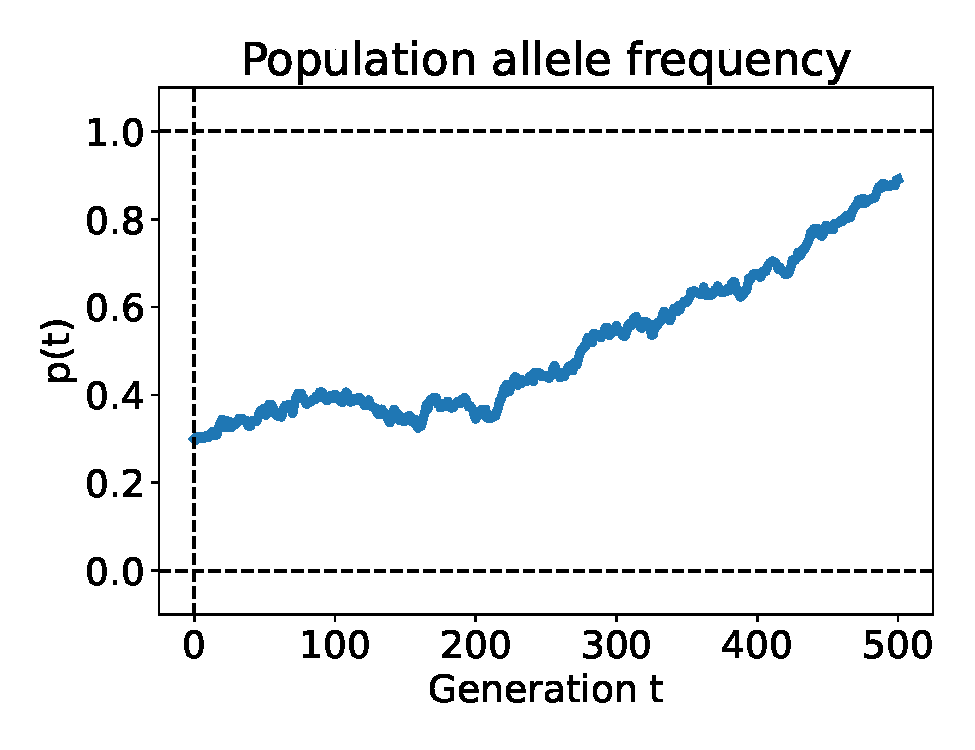
\includegraphics[width=.8\textwidth]{graphics/one_diffusion.pdf}
        \end{column}
        \begin{column}{0.5\textwidth}
            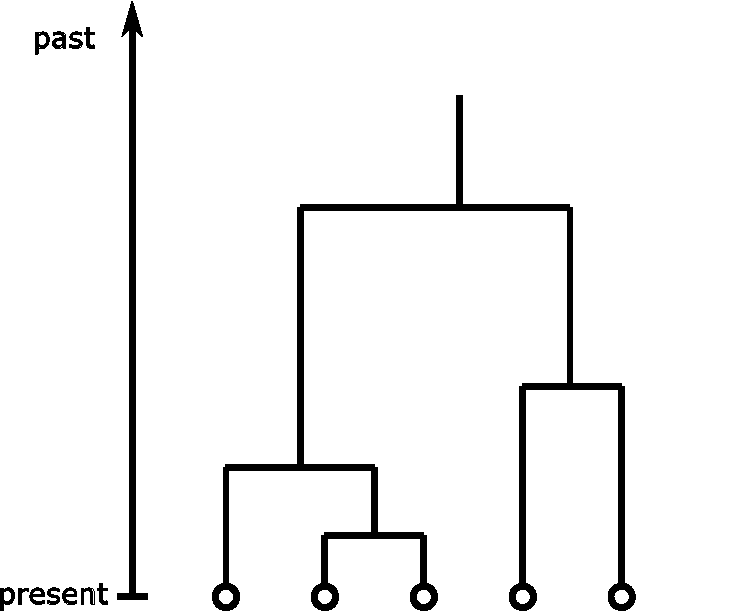
\includegraphics[width=.8\textwidth]{graphics/coalescent_tree.pdf}
        \end{column}
    \end{columns}
\end{frame}
%%%%%%%%%%%%%%%%%%%%%%%%%%%%%%%%%%%%%%%%%%%%%%%%%%%%%%%%%%%%%%%%%%%%%%%%%%%%%%%%%%%%%%
%
%
%
%%%%%%%%%%%%%%%%%%%%%%%%%%%%%%%%%%%%%%%%%%%%%%%%%%%%%%%%%%%%%%%%%%%%%%%%%%%%%%%%%%%%%%
\begin{frame}{Probability and statistics}
    \begin{itemize}
        \item Population genetic processes are random.
        \begin{itemize}
            % \item Or very complex, so modelling as random might be easier.
            \item Need models for randomness.
        \end{itemize}
        \item Statistics needed for analyzing (genomic) data.
        \begin{itemize}
            \item Analyze genomic data of (randomly) sampled individuals.
            \item Handle sampling/measurement uncertainty.
        \end{itemize}
    \end{itemize}
    \begin{block}{}
        \begin{itemize}
            \item[$\to$] Probability and statistics essential for population genomics. 
        \end{itemize}
    \end{block}
\end{frame}
%%%%%%%%%%%%%%%%%%%%%%%%%%%%%%%%%%%%%%%%%%%%%%%%%%%%%%%%%%%%%%%%%%%%%%%%%%%%%%%%%%%%%%
%
%
%
%%%%%%%%%%%%%%%%%%%%%%%%%%%%%%%%%%%%%%%%%%%%%%%%%%%%%%%%%%%%%%%%%%%%%%%%%%%%%%%%%%%%%%
\begin{frame}{Note}
    \begin{itemize}
        \item I will present some background.
        \item Helpful preparation for the remainder of the course.
        \item Not possible to cover every detail.
        \item If you are familiar with most of these topics, that's good.
        \item If not, possibly read up on some before the course starts.
        \begin{itemize}
            \item Many accessible textbooks cover these topics.
            \item I'd be happy to provide additional material/pointers.
            \item Feel free to reach out via email: \texttt{steinrue@uchicago.edu}.
            \item Or on slack.
        \end{itemize}
    \end{itemize}
\end{frame}
%%%%%%%%%%%%%%%%%%%%%%%%%%%%%%%%%%%%%%%%%%%%%%%%%%%%%%%%%%%%%%%%%%%%%%%%%%%%%%%%%%%%%%
%
%
%
% %%%%%%%%%%%%%%%%%%%%%%%%%%%%%%%%%%%%%%%%%%%%%%%%%%%%%%%%%%%%%%%%%%%%%%%%%%%%%%%%%%%%%%
% \begin{frame}{Deterministic models}
%     \begin{block}{}
%         How does genetic variation change forward-in-time?
%     \end{block}
%     Very simple model:
%     \begin{itemize}
%         \item Single genetic locus.
%         \item Two possible alleles/genetic variants: \text{a} or \text{A}.
%         \item Track $p(t)$, population allele frequency of allele \text{A} in generation $t$.
%         \begin{itemize}
%             \item That is, what fraction of individuals in population has allele \text{A}.
%         \end{itemize}
%     \end{itemize}
% \end{frame}
% %%%%%%%%%%%%%%%%%%%%%%%%%%%%%%%%%%%%%%%%%%%%%%%%%%%%%%%%%%%%%%%%%%%%%%%%%%%%%%%%%%%%%%
% %
% %
% %
% %%%%%%%%%%%%%%%%%%%%%%%%%%%%%%%%%%%%%%%%%%%%%%%%%%%%%%%%%%%%%%%%%%%%%%%%%%%%%%%%%%%%%%
% \begin{frame}{Ordinary differential equation}
%     \begin{block}{}
%         How does genetic variation change forward-in-time?
%     \end{block}
%     Specify change from one generation to next
%     \begin{block}{Ordinary differential equation (ODE)}
%         \begin{itemize}
%             \item Using derivative in time: $\tfrac{d}{dt}p(t)$.
%         \end{itemize}
%     \end{block}
%     Frequency in next generation:
%     \begin{equation}
%         p(t+1) \approx p(t) + \tfrac{d}{dt}p(t)
%     \end{equation}
%     \begin{itemize}
%         \item Sign of $\tfrac{d}{dt}p(t)$ determines whether $p(t)$ increases or decreases.
%         \item Magnitude determines by how much.
%     \end{itemize}
% \end{frame}
% %%%%%%%%%%%%%%%%%%%%%%%%%%%%%%%%%%%%%%%%%%%%%%%%%%%%%%%%%%%%%%%%%%%%%%%%%%%%%%%%%%%%%%
% %
% %
% %
% %%%%%%%%%%%%%%%%%%%%%%%%%%%%%%%%%%%%%%%%%%%%%%%%%%%%%%%%%%%%%%%%%%%%%%%%%%%%%%%%%%%%%%
% \begin{frame}{Example: Additive selection}
%     Assume:
%     \begin{itemize}
%         \item Allele \text{a} confers baseline fitness $1$.
%         \item Allele \text{A} confers fitness $1+s$.
%     \end{itemize}
%     In this case:
%     \begin{equation}
%         \tfrac{d}{dt}p(t) = sp(1-p)
%     \end{equation}
%     \begin{itemize}
%         \item Can actually be solved analytically:
%     \end{itemize}
%     \begin{equation}
%         p(t) = \frac{e^{st}p(0)}{(1-p(0)) + e^{st}p(0)}
%     \end{equation}
%     \begin{itemize}
%         \item \textcolor{red}{Draw tangents in plot}?
%         \begin{itemize}
%             \item Maybe even step by step.
%         \end{itemize}
%     \end{itemize}
%     \begin{center}
%         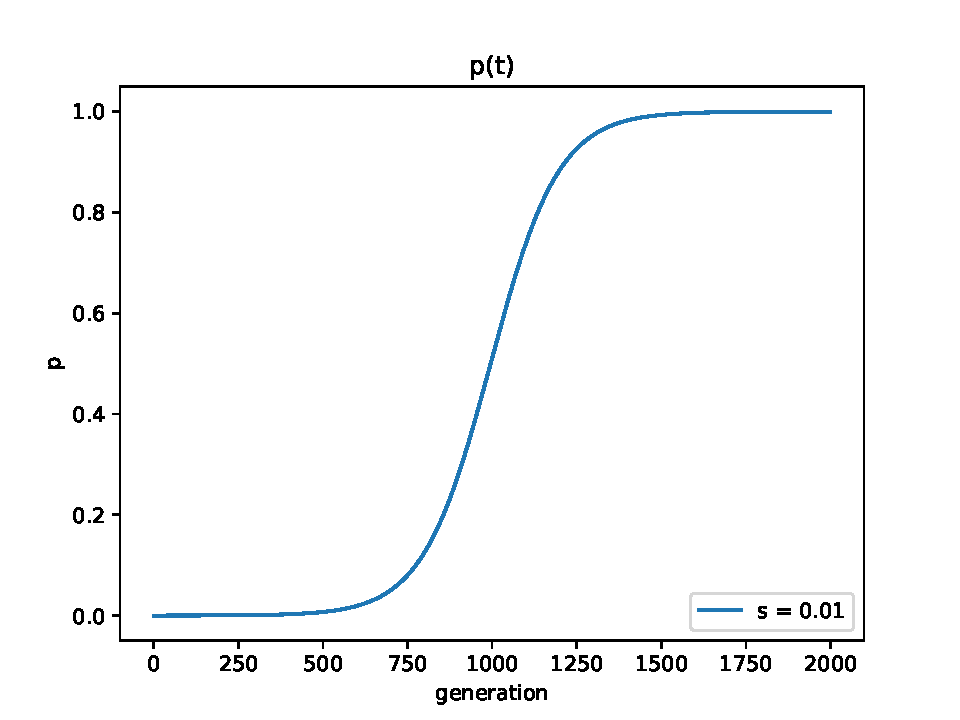
\includegraphics[width=.5\textwidth]{graphics/selection_trajectory.pdf}
%     \end{center}
%     \begin{itemize}
%         \item In finite populations: Beneficial allele can be lost (random).
%     \end{itemize}
% \end{frame}
% %%%%%%%%%%%%%%%%%%%%%%%%%%%%%%%%%%%%%%%%%%%%%%%%%%%%%%%%%%%%%%%%%%%%%%%%%%%%%%%%%%%%%%
% %
% %
% %
% %%%%%%%%%%%%%%%%%%%%%%%%%%%%%%%%%%%%%%%%%%%%%%%%%%%%%%%%%%%%%%%%%%%%%%%%%%%%%%%%%%%%%%
% \begin{frame}{Solving ODEs}
%     \begin{itemize}
%         \item Full analytic solution often only possible in simple cases.
%         \item If not possible, can still make quantitative statements.
%         \begin{itemize}
%             \item E.g.\ If $\tfrac{d}{dt}p(t) > 0$, then $p(t)$ will increase.
%         \end{itemize}
%         \item Many methods to obtain numerical solutions:
%         \begin{itemize}
%             \item In \texttt{R}: Packages \texttt{deSolve}, \texttt{pracma}.
%             \item In \texttt{Python}: Function \texttt{scipy.integrate.odeint}.
%         \end{itemize}
%     \end{itemize}
% \end{frame}
% %%%%%%%%%%%%%%%%%%%%%%%%%%%%%%%%%%%%%%%%%%%%%%%%%%%%%%%%%%%%%%%%%%%%%%%%%%%%%%%%%%%%%%
%
%
%
% %%%%%%%%%%%%%%%%%%%%%%%%%%%%%%%%%%%%%%%%%%%%%%%%%%%%%%%%%%%%%%%%%%%%%%%%%%%%%%%%%%%%%%
% \begin{frame}{Probability and Statistics}
%     \begin{itemize}
%         \item Many population genetic processes involve randomness.
%         \item Or are so complicated that modelling them as random is easier.
%     \end{itemize}
%     Thus, we will go over some basic probability.
% \end{frame}
% %%%%%%%%%%%%%%%%%%%%%%%%%%%%%%%%%%%%%%%%%%%%%%%%%%%%%%%%%%%%%%%%%%%%%%%%%%%%%%%%%%%%%%
% %
% %
% %
% %%%%%%%%%%%%%%%%%%%%%%%%%%%%%%%%%%%%%%%%%%%%%%%%%%%%%%%%%%%%%%%%%%%%%%%%%%%%%%%%%%%%%%
% \begin{frame}{Random variables}
%     \textcolor{red}{DON'T INTRODUCE RANDOM VARIABLES.}
%     Essentially:
%     \begin{block}{Random variable $X$}
%         Describes a random event/outcome.
%     \end{block}
%     \begin{itemize}
%         \item Math.\ def.\ more involved, but not relevant for everyday life.
%     \end{itemize}
%     Need to define two things:
%     \begin{enumerate}
%         \item Possible outcomes.
%         \item Probabilities of those outcomes.
%     \end{enumerate}
% \end{frame}
% %%%%%%%%%%%%%%%%%%%%%%%%%%%%%%%%%%%%%%%%%%%%%%%%%%%%%%%%%%%%%%%%%%%%%%%%%%%%%%%%%%%%%%
%
%
%
%%%%%%%%%%%%%%%%%%%%%%%%%%%%%%%%%%%%%%%%%%%%%%%%%%%%%%%%%%%%%%%%%%%%%%%%%%%%%%%%%%%%%%
\begin{frame}{Probability distributions}
    \begin{block}{Example: Throw a die.}
        \begin{enumerate}
        \item Outcomes: 1, 2, ..., 6.
            \begin{itemize}
                \item $X \in \{1,2,\ldots,6\}$.
            \end{itemize}
        \item Probabilities: Every number with equal probability.
            \begin{itemize}
                \item $\P\{X = 1\} = \P\{X = 2\} = \ldots = \P\{X = 6\} = \tfrac{1}{6}$.
            \end{itemize}
        \end{enumerate}
    \end{block}
    \begin{columns}
        \begin{column}{.5\textwidth}
            \begin{center}
                
\includegraphics[width=.8\textwidth]{graphics/uniform_die.pdf}
            \end{center}
        \end{column}
        \begin{column}{.5\textwidth}
            \begin{center}
                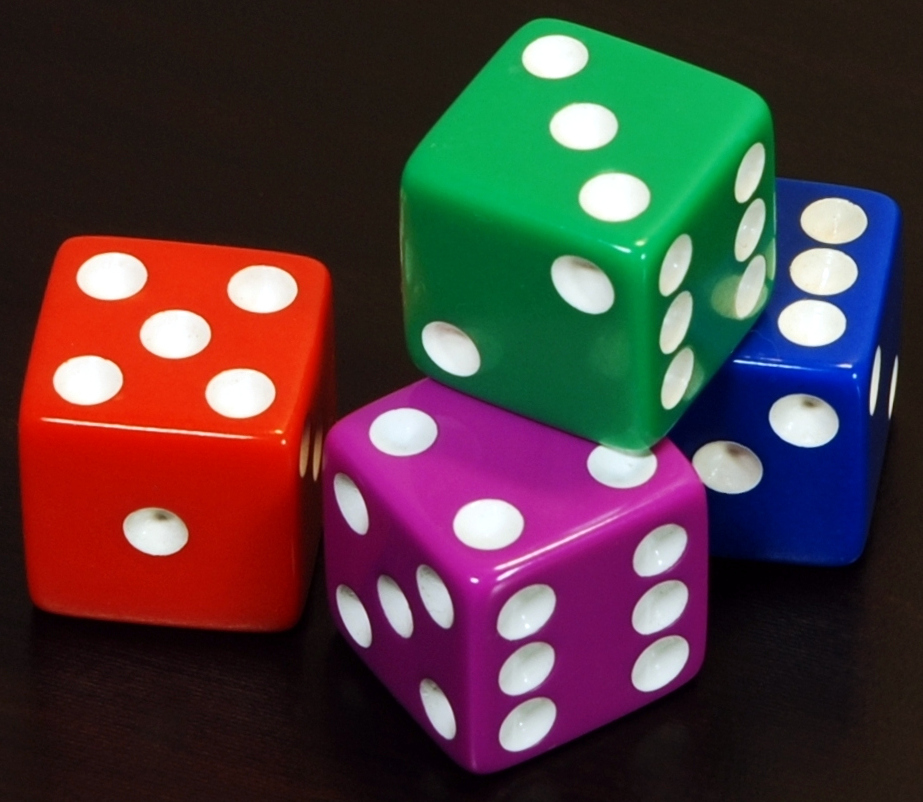
\includegraphics[width=.5\textwidth]{graphics/6sided_dice_(cropped).jpg}\\\tiny{\url{https://en.wikipedia.org/wiki/Dice}}
            \end{center}
        \end{column}
    \end{columns}
    \begin{itemize}
        % \item ``Probabilities'' also called ``distribution''.
        \item Often shorthand notation: $p_i := \P\{X=i\} \geq 0$.
        \item Have to sum to one: $\sum_{\text{all outcomes }k} p_k = 1$.
    \end{itemize}
\end{frame}
%%%%%%%%%%%%%%%%%%%%%%%%%%%%%%%%%%%%%%%%%%%%%%%%%%%%%%%%%%%%%%%%%%%%%%%%%%%%%%%%%%%%%%
%
%
%
%%%%%%%%%%%%%%%%%%%%%%%%%%%%%%%%%%%%%%%%%%%%%%%%%%%%%%%%%%%%%%%%%%%%%%%%%%%%%%%%%%%%%%
\begin{frame}{Expected value}
    \begin{block}{Expected value}
        If I receive as many Euros as the die shows pips, then how much money should I expect.
    \end{block}
    \begin{columns}
        \begin{column}{.65\textwidth}
            \begin{itemize}
                \item 1 pip w.p.\ $p_1$.
                \item 2 pips w.p.\ $p_2$.
                \item ...
                \item 6 pips w.p.\ $p_6$.
            \end{itemize}
            I get $k$ Euro ($k$ pips) with probability $p_k$.
        \end{column}
        \begin{column}{.35\textwidth}
            \begin{center}
                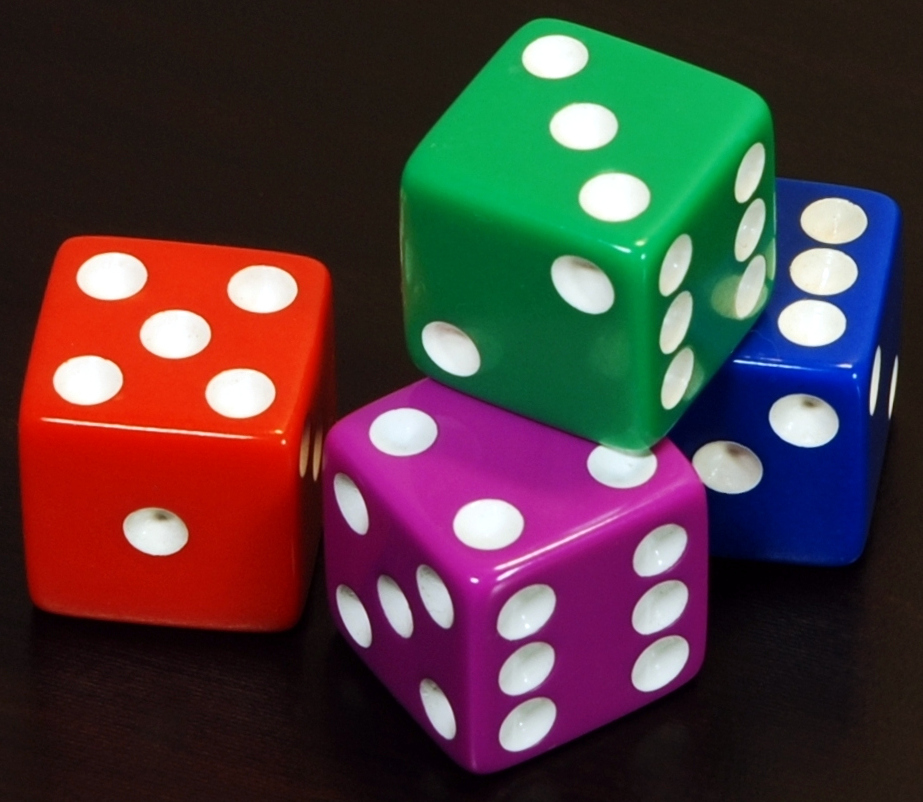
\includegraphics[width=.85\textwidth]{graphics/6sided_dice_(cropped).jpg}\\\tiny{\url{https://en.wikipedia.org/wiki/Dice}}
            \end{center}
        \end{column}
    \end{columns}
    In general:
    \begin{block}{}
        \begin{equation}
            \E [X] := \sum_{\text{all outcomes }k} k \cdot p_k
        \end{equation}
    \end{block}
    Specifically for one die: $\E[X] = 3.5$.
\end{frame}
%%%%%%%%%%%%%%%%%%%%%%%%%%%%%%%%%%%%%%%%%%%%%%%%%%%%%%%%%%%%%%%%%%%%%%%%%%%%%%%%%%%%%%
%
%
%
%%%%%%%%%%%%%%%%%%%%%%%%%%%%%%%%%%%%%%%%%%%%%%%%%%%%%%%%%%%%%%%%%%%%%%%%%%%%%%%%%%%%%%
\begin{frame}{Empirical mean}
    \begin{block}{}
        Unknown distribution of $X$.
        \begin{itemize}
            \item Estimate the expected value using the empirical mean.
        \end{itemize}
    \end{block}
    \begin{itemize}
        \item Repeat random experiment $L$ times, and average outcomes.
    \end{itemize}
    Outcome of replicate $i$: $X^{(i)}$.
    \begin{block}{Empirical mean}
        \begin{equation}
            \bar{X} := \tfrac{1}{L} \sum_{i=1}^L X^{(i)}
        \end{equation}
    \end{block}
    $\bar{X}$ is an estimate of $\E[X]$:
    \begin{equation}
        \E[X] \approx \bar{X}.
    \end{equation}
\end{frame}
%%%%%%%%%%%%%%%%%%%%%%%%%%%%%%%%%%%%%%%%%%%%%%%%%%%%%%%%%%%%%%%%%%%%%%%%%%%%%%%%%%%%%%
%
%
%
%%%%%%%%%%%%%%%%%%%%%%%%%%%%%%%%%%%%%%%%%%%%%%%%%%%%%%%%%%%%%%%%%%%%%%%%%%%%%%%%%%%%%%
\begin{frame}{Variance}
    \begin{block}{}
        How much does outcome vary around the expected value?
    \end{block}
    Variance: Expected squared deviation from mean.
    \begin{block}{Variance}
        \begin{equation}
            \V [X] := \sum_{\text{all outcomes }k} \big(k - \E[X]\big)^2 \cdot p_k
        \end{equation}
    \end{block}
    \begin{itemize}
        \item Small variance: Outcome will be close to expected value.
        \item Large variance: Large spread of possible values.
        \item Important when dealing with uncertainty, risk management.
    \end{itemize}
    \begin{block}{Standard deviation}
        \begin{equation}
            \sigma_X := \sqrt{\V[X]}
        \end{equation}
    \end{block}
\end{frame}
%%%%%%%%%%%%%%%%%%%%%%%%%%%%%%%%%%%%%%%%%%%%%%%%%%%%%%%%%%%%%%%%%%%%%%%%%%%%%%%%%%%%%%
%
%
%
%%%%%%%%%%%%%%%%%%%%%%%%%%%%%%%%%%%%%%%%%%%%%%%%%%%%%%%%%%%%%%%%%%%%%%%%%%%%%%%%%%%%%%
\begin{frame}{Common discrete probability distributions}
    Frequently used basic discrete probability distributions:
    \begin{itemize}
        % \item Bernoulli?
        \item Binomial distribution.
        \item Geometric distribution.
        \item Poisson distribution.
    \end{itemize}
\end{frame}
%%%%%%%%%%%%%%%%%%%%%%%%%%%%%%%%%%%%%%%%%%%%%%%%%%%%%%%%%%%%%%%%%%%%%%%%%%%%%%%%%%%%%%
%
%
%
%%%%%%%%%%%%%%%%%%%%%%%%%%%%%%%%%%%%%%%%%%%%%%%%%%%%%%%%%%%%%%%%%%%%%%%%%%%%%%%%%%%%%%
\begin{frame}{Binomial distribution}
    \begin{itemize}
        \item Consider flipping a coin $n$ times.
        \item Coin has probability $p$ to come up heads.
        \item Probability $(1-p)$ to come up tails.
    \end{itemize}
    \begin{block}{Binomial distribution}
        Describes the number of times the coin comes up heads.
    \end{block}$~$\\[-4.5ex]
    \begin{equation}
        \P\{X = k\} = \tfrac{n!}{k!(n-k)!} p^k(1-p)^{n-k}
    \end{equation}\\[-2ex]
    \begin{columns}
        \begin{column}{.5\textwidth}
            \begin{center}
                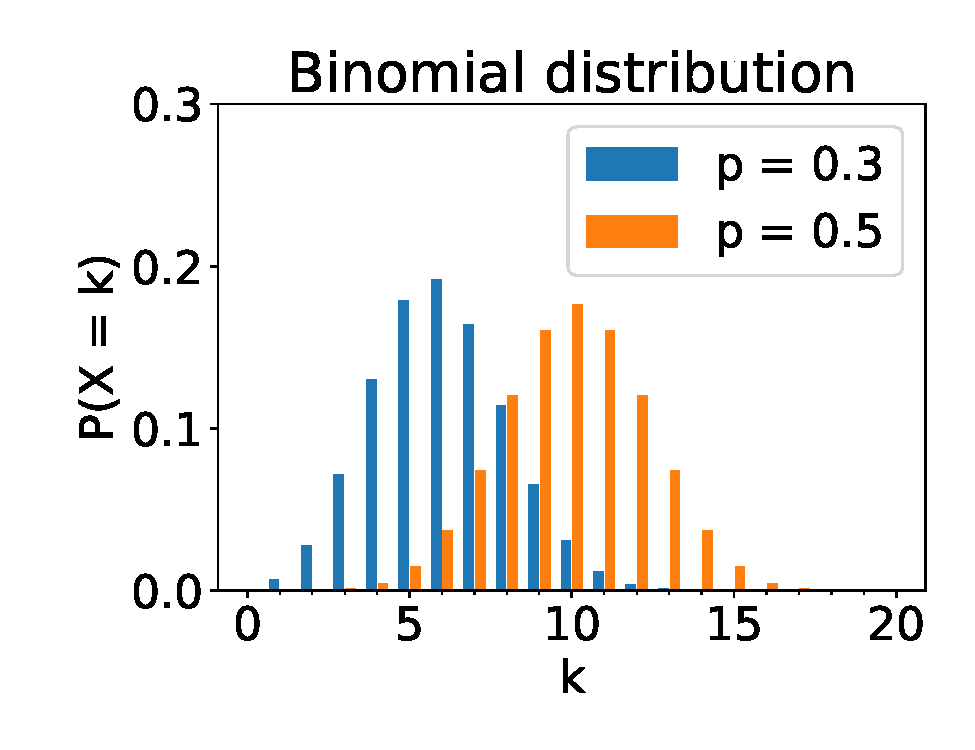
\includegraphics[width=\textwidth]{graphics/binomial_distribution.pdf}
            \end{center}
        \end{column}
        \begin{column}{.5\textwidth}
            \begin{center}
                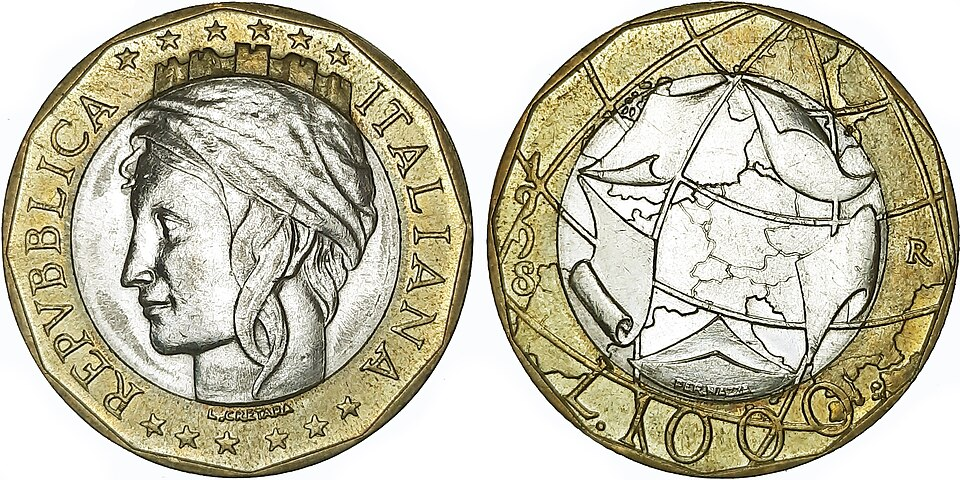
\includegraphics[width=.9\textwidth]{graphics/960px-1000_lire.jpg}\\\tiny{\url{https://en.wikipedia.org/wiki/Italian_lira}}
            \end{center}
        \end{column}
    \end{columns}
\end{frame}
%%%%%%%%%%%%%%%%%%%%%%%%%%%%%%%%%%%%%%%%%%%%%%%%%%%%%%%%%%%%%%%%%%%%%%%%%%%%%%%%%%%%%%
%
%
%
%%%%%%%%%%%%%%%%%%%%%%%%%%%%%%%%%%%%%%%%%%%%%%%%%%%%%%%%%%%%%%%%%%%%%%%%%%%%%%%%%%%%%%
\begin{frame}{Binomial distribution}
    \begin{block}{}
        \begin{equation}
            X \sim \text{Bin}(n,p)
        \end{equation}
    \end{block}
    \begin{equation}
        \E [X] = np \qquad \text{and} \qquad \V [X] = np(1-p)
    \end{equation}
    \begin{block}{Example: Wright-Fisher model}
        \begin{itemize}
            \item Offspring inherits alleles from parents.
            \item Number of alleles in next generation is binomially distributed.
        \end{itemize}
    \end{block}
\end{frame}
%%%%%%%%%%%%%%%%%%%%%%%%%%%%%%%%%%%%%%%%%%%%%%%%%%%%%%%%%%%%%%%%%%%%%%%%%%%%%%%%%%%%%%
%
%
%
%%%%%%%%%%%%%%%%%%%%%%%%%%%%%%%%%%%%%%%%%%%%%%%%%%%%%%%%%%%%%%%%%%%%%%%%%%%%%%%%%%%%%%
\begin{frame}{Geometric distribution}
    \begin{itemize}
        \item Consider flipping a coin.
        \item Each coin has probability $p$ to come up heads.
    \end{itemize}
    \begin{block}{Geometric distribution}
        How many times do I have to flip until I see \textbf{head} the first time?
    \end{block}
    \begin{equation}
        \P\{X = k\} = (1-p)^{k-1}p
    \end{equation}
    \begin{center}
        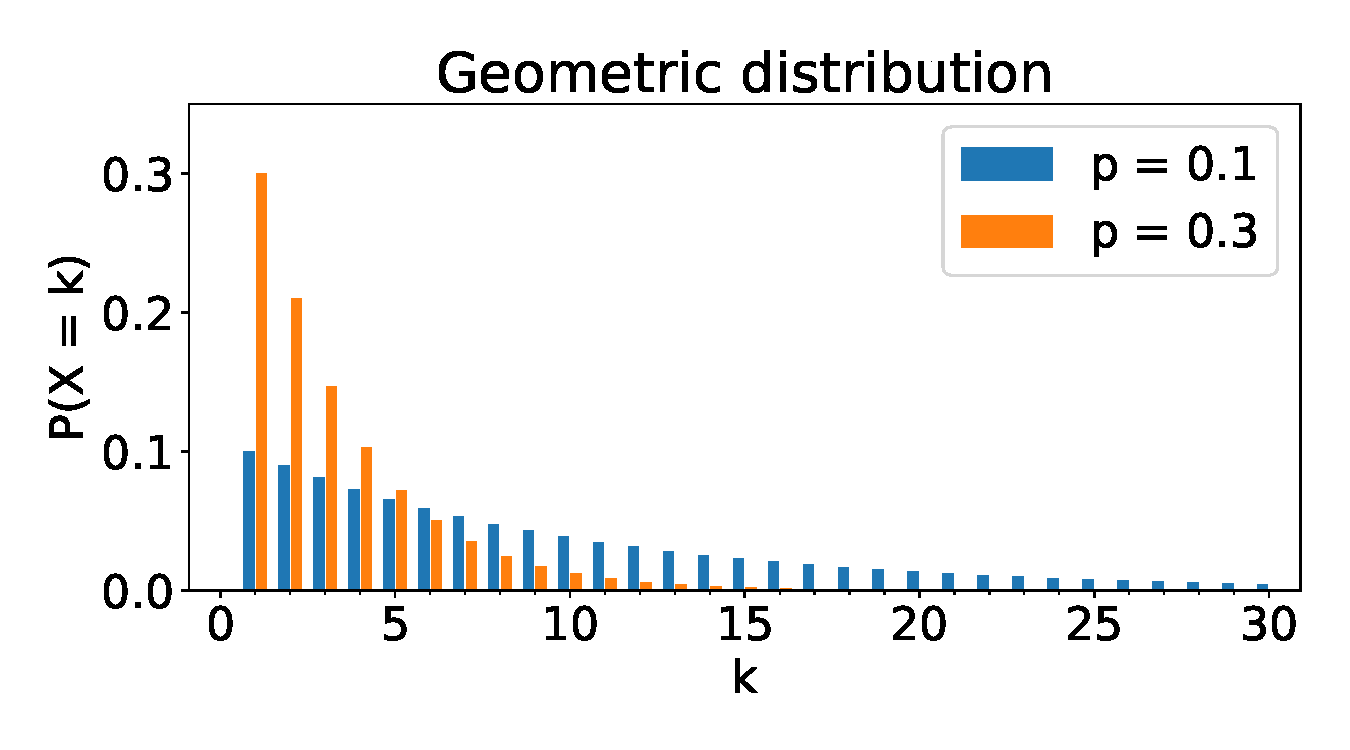
\includegraphics[width=.7\textwidth]{graphics/geometric_distribution.pdf}
    \end{center}$~$\\[-6ex]
    \begin{itemize}
        \item \textbf{Waiting time}.
    \end{itemize}
\end{frame}
%%%%%%%%%%%%%%%%%%%%%%%%%%%%%%%%%%%%%%%%%%%%%%%%%%%%%%%%%%%%%%%%%%%%%%%%%%%%%%%%%%%%%%
%
%
%
%%%%%%%%%%%%%%%%%%%%%%%%%%%%%%%%%%%%%%%%%%%%%%%%%%%%%%%%%%%%%%%%%%%%%%%%%%%%%%%%%%%%%%
\begin{frame}{Geometric distribution}
    \begin{center}
        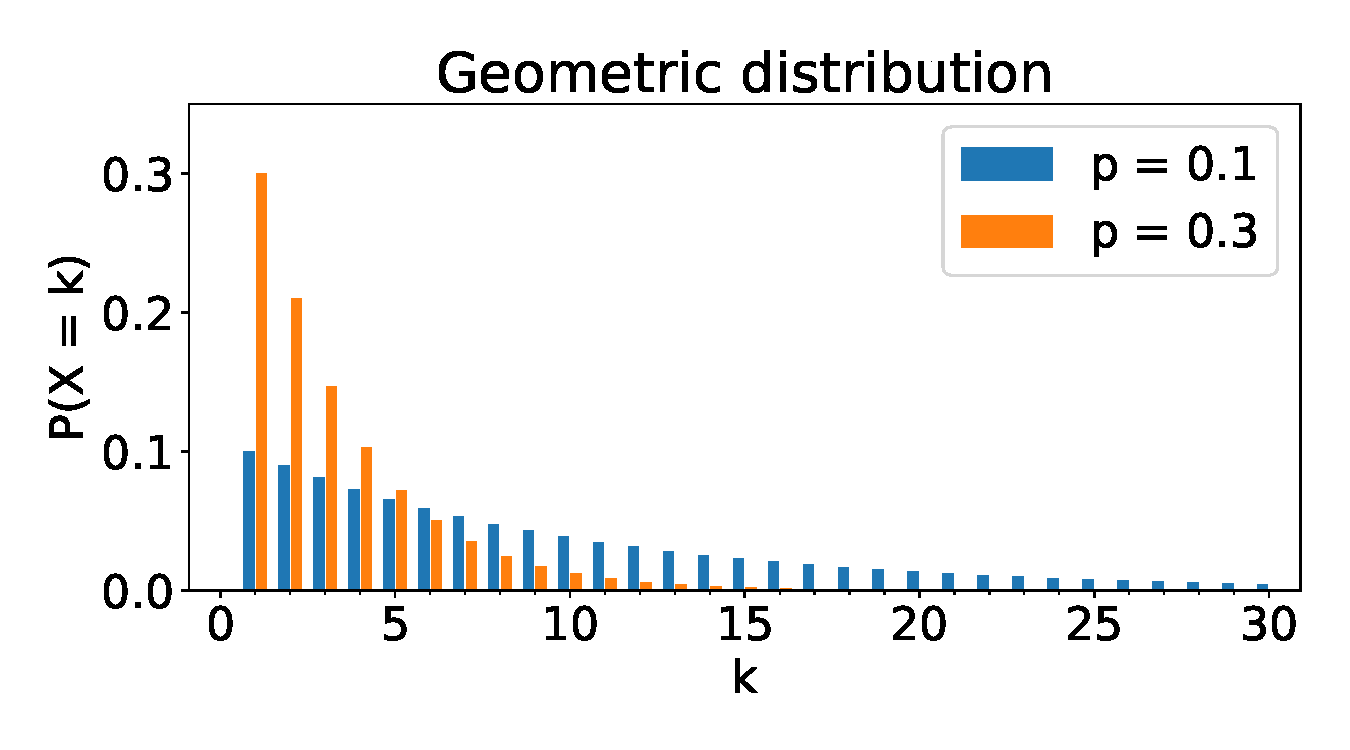
\includegraphics[width=.5\textwidth]{graphics/geometric_distribution.pdf}
    \end{center}$~$\\[-5ex]
    \begin{block}{}
        \begin{equation}
            X \sim \text{Geom}(p)
        \end{equation}
    \end{block}$~$\\[-5ex]
    \begin{equation}
        \E [X] = \tfrac{1}{p} \qquad \text{and} \qquad \V [X] = \tfrac{1-p}{p^2}
    \end{equation}$~$\\[-3ex]
    \begin{block}{Example: Time to most recent common ancestor}
        \begin{itemize}
            \item Two haploids in population of size $2N$.
            \item Prob.\ that common parent in previous gener.: $\tfrac{1}{2N}$.
            \item \# gener. to most recent common ancestor $\sim \text{Geom}(\tfrac{1}{2N})$.
            \item Expected \# gener.\ until most recent common ancestor $2N$.
        \end{itemize}
    \end{block}
\end{frame}
%%%%%%%%%%%%%%%%%%%%%%%%%%%%%%%%%%%%%%%%%%%%%%%%%%%%%%%%%%%%%%%%%%%%%%%%%%%%%%%%%%%%%%
%
%
%
%%%%%%%%%%%%%%%%%%%%%%%%%%%%%%%%%%%%%%%%%%%%%%%%%%%%%%%%%%%%%%%%%%%%%%%%%%%%%%%%%%%%%%
\begin{frame}{Poisson distribution}
    \begin{itemize}
        \item Number of events in a given time interval.
        \item Expected number of events: $\mu$.
    \end{itemize}
    \begin{block}{Poisson distribution}
        \begin{equation}
            \P\{X = k\} = \tfrac{\mu^k e^{-k}}{k!}
        \end{equation}
    \end{block}
    \begin{center}
        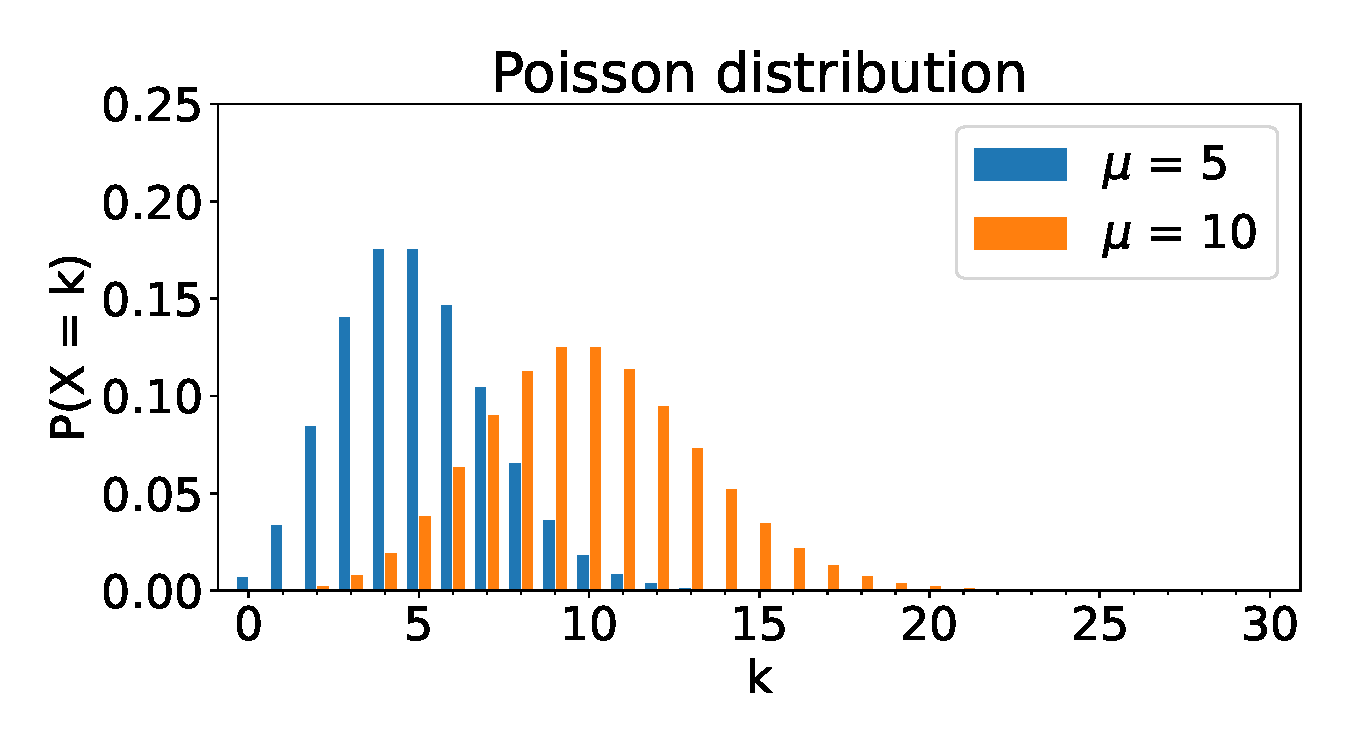
\includegraphics[width=.7\textwidth]{graphics/poisson_distribution.pdf}
    \end{center}
\end{frame}
%%%%%%%%%%%%%%%%%%%%%%%%%%%%%%%%%%%%%%%%%%%%%%%%%%%%%%%%%%%%%%%%%%%%%%%%%%%%%%%%%%%%%%
%
%
%
%%%%%%%%%%%%%%%%%%%%%%%%%%%%%%%%%%%%%%%%%%%%%%%%%%%%%%%%%%%%%%%%%%%%%%%%%%%%%%%%%%%%%%
\begin{frame}{Poisson distribution}
    % \begin{center}
    %     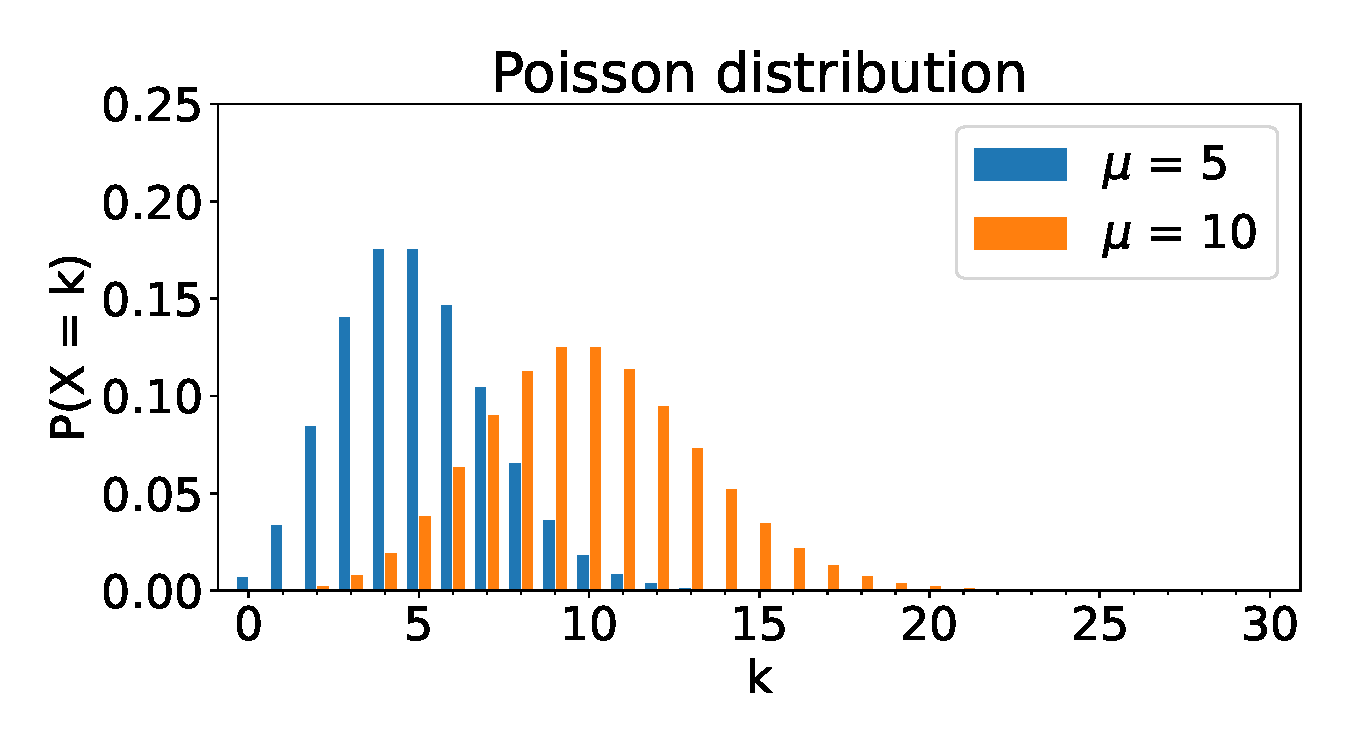
\includegraphics[width=.5\textwidth]{graphics/poisson_distribution.pdf}
    % \end{center}$~$\\[-5ex]
    \begin{block}{}
        \begin{equation}
            X \sim \text{Poisson}(\mu)
        \end{equation}
    \end{block}$~$\\[-5ex]
    \begin{equation}
        \E [X] = \mu \qquad \text{and} \qquad \V [X] = \mu
    \end{equation}$~$\\[-3ex]
    \begin{block}{Example: Number of mutations on evolutionary branches}
        \begin{itemize}
            \item Consider gene with $L = 10,000$ bp.
            \item Per generation per bp mutation prob $u = 10^{-8}$.
            \item Human-Chimp divergence time $T = 250,000$ generations.
            \item \# mutations in gene between Human-Chimp $\sim \text{Poisson}(\mu)$.
            \item With $\mu := L \cdot u \cdot 2T = 25$ (expected value).
        \end{itemize}
    \end{block}
\end{frame}
%%%%%%%%%%%%%%%%%%%%%%%%%%%%%%%%%%%%%%%%%%%%%%%%%%%%%%%%%%%%%%%%%%%%%%%%%%%%%%%%%%%%%%
% 
%
%
%%%%%%%%%%%%%%%%%%%%%%%%%%%%%%%%%%%%%%%%%%%%%%%%%%%%%%%%%%%%%%%%%%%%%%%%%%%%%%%%%%%%%%
\begin{frame}{Continuous probability distributions}
    We had:
    \begin{itemize}
        \item Discrete probability distributions.
        \item Used to model discrete outcomes:
        \begin{itemize}
            \item Number of mutations.
            \item Number of generations.
            \item Number of alleles.
            \item ...
        \end{itemize}
    \end{itemize}
    However, some quantities/measurements are on continuous scales:
    \begin{itemize}
        \item Height
        \item Wingspan
        \item Cholesterol level
        \item ...
    \end{itemize}
    \begin{block}{}
        Need continuous probability distributions.
    \end{block}
\end{frame}
%%%%%%%%%%%%%%%%%%%%%%%%%%%%%%%%%%%%%%%%%%%%%%%%%%%%%%%%%%%%%%%%%%%%%%%%%%%%%%%%%%%%%%
%
%
%
%%%%%%%%%%%%%%%%%%%%%%%%%%%%%%%%%%%%%%%%%%%%%%%%%%%%%%%%%%%%%%%%%%%%%%%%%%%%%%%%%%%%%%
\begin{frame}{Continuous probability distributions}
    Discrete distributions:
    \begin{itemize}
        \item We defined probability $p_k$ for every outcome $k$.
    \end{itemize}
    Continuous distributions:
    \begin{itemize}
        \item Can't define probability for each outcome (technical reasons).
        \item Rather, introduce:
    \end{itemize}
    \begin{block}{}
         \textbf{Probability density function} (pdf): $f(x)$.
    \end{block}
    \begin{itemize}
        \item $f(x) \geq 0$ gives likelihood of outcome $x \in \R$.
        \item Has to integrate to 1: $\int_{-\infty}^\infty f(x) dx = 1$.
    \end{itemize}
    \begin{center}
        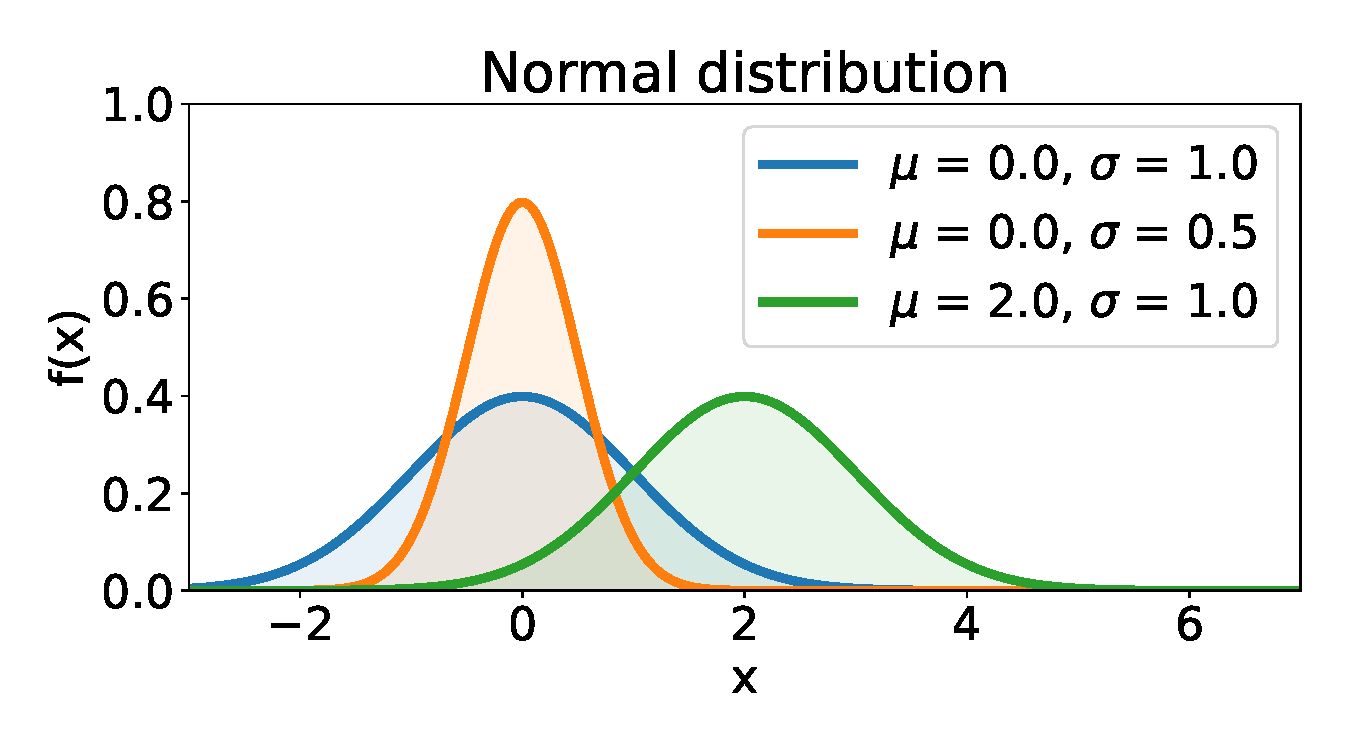
\includegraphics[width=.5\textwidth]{graphics/normal_distribution.pdf}
    \end{center}
\end{frame}
%%%%%%%%%%%%%%%%%%%%%%%%%%%%%%%%%%%%%%%%%%%%%%%%%%%%%%%%%%%%%%%%%%%%%%%%%%%%%%%%%%%%%%
%
%
%
%%%%%%%%%%%%%%%%%%%%%%%%%%%%%%%%%%%%%%%%%%%%%%%%%%%%%%%%%%%%%%%%%%%%%%%%%%%%%%%%%%%%%%
\begin{frame}{Expected value \& variance}
    \begin{block}{}
        Same interpretation as in discrete case:
    \end{block}
    \begin{itemize}
        \item Expected value: Expected outcome.
        \item Variance: Spread around expected outcome.
    \end{itemize}
    However, replace discrete sum with continuous integral:
    \begin{block}{}
        \begin{equation}
            \E[X] := \int_{-\infty}^\infty x \cdot f(x) dx
        \end{equation}
    \end{block}
    and
    \begin{block}{}
        \begin{equation}
            \V[X] := \int_{-\infty}^\infty (x - \E[X])^2 \cdot f(x) dx
        \end{equation}
    \end{block}
    \begin{itemize}
        \item If limited range, adjust integral boundaries.
    \end{itemize}
\end{frame}
%%%%%%%%%%%%%%%%%%%%%%%%%%%%%%%%%%%%%%%%%%%%%%%%%%%%%%%%%%%%%%%%%%%%%%%%%%%%%%%%%%%%%%
%
%
%
%%%%%%%%%%%%%%%%%%%%%%%%%%%%%%%%%%%%%%%%%%%%%%%%%%%%%%%%%%%%%%%%%%%%%%%%%%%%%%%%%%%%%%
\begin{frame}{Common continuous distributions}
    Frequently used continuous distributions:
    \begin{itemize}
        \item Uniform.
        \item Normal distribution.
        \item Exponential distribution.
        \item Beta distribution.
    \end{itemize}
\end{frame}
%%%%%%%%%%%%%%%%%%%%%%%%%%%%%%%%%%%%%%%%%%%%%%%%%%%%%%%%%%%%%%%%%%%%%%%%%%%%%%%%%%%%%%
%
%
%
%%%%%%%%%%%%%%%%%%%%%%%%%%%%%%%%%%%%%%%%%%%%%%%%%%%%%%%%%%%%%%%%%%%%%%%%%%%%%%%%%%%%%%
\begin{frame}{Uniform distribution}
    \begin{block}{}
        All values between lower bound $a$ and upper bound $b$ equally likely.
    \end{block}
    \begin{equation}
        X \sim \text{Unif[a,b]}
    \end{equation}$~$\\[-3ex]
    \begin{equation}
        f(x) = \begin{cases}
            \tfrac{1}{b-a}, & \text{if $a \leq x \leq b$},\\
            0, & \text{otherwise}.
        \end{cases}
    \end{equation}
    \begin{center}
        
\includegraphics[width=.7\textwidth]{graphics/uniform_density.pdf}
    \end{center}
\end{frame}
%%%%%%%%%%%%%%%%%%%%%%%%%%%%%%%%%%%%%%%%%%%%%%%%%%%%%%%%%%%%%%%%%%%%%%%%%%%%%%%%%%%%%%
%
%
%
%%%%%%%%%%%%%%%%%%%%%%%%%%%%%%%%%%%%%%%%%%%%%%%%%%%%%%%%%%%%%%%%%%%%%%%%%%%%%%%%%%%%%%
\begin{frame}{Normal distribution}
    Very common, flexible distribution:
    \begin{itemize}
        \item Determined by mean $\mu$ and standard deviation $\sigma$ (or variance).
    \end{itemize}
    \begin{block}{}
        \begin{equation}
            X \sim \text{Norm}(\mu, \sigma), \qquad f(x) = \tfrac{1}{\sqrt{2\pi\sigma^2}} \exp \big( \tfrac{(x-\mu)^2}{2\sigma^2}\big)
        \end{equation}
    \end{block}$~$\\[-6ex]$~$
    \begin{center}
        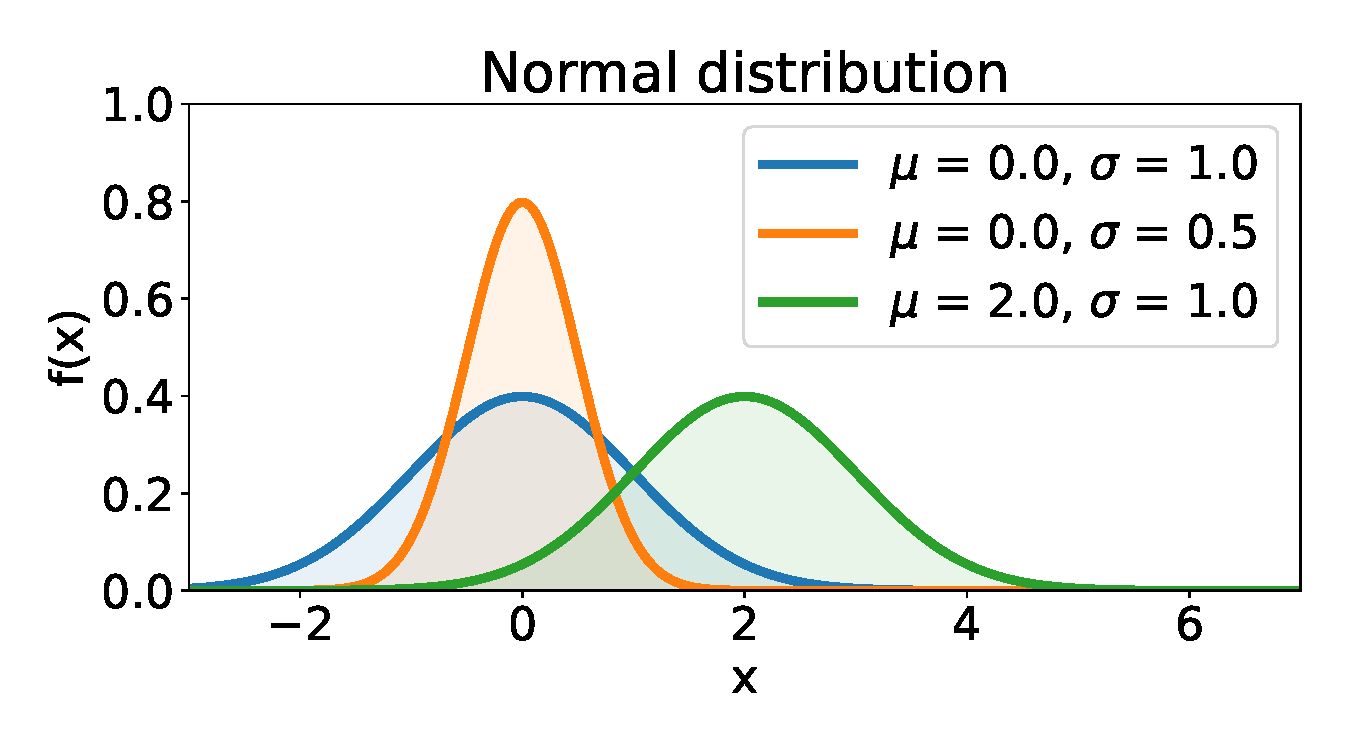
\includegraphics[width=.7\textwidth]{graphics/normal_distribution.pdf}
    \end{center}$~$\\[-8ex]
    \begin{equation}
        \text{Surprise:} \qquad \E[X] = \mu \qquad \text{and} \qquad \V[X] = \sigma^2
    \end{equation}$~$\\[-2ex]
    \begin{itemize}
        \item Sum of many small contributions approx.\ normal distributed.
    \end{itemize}
\end{frame}
%%%%%%%%%%%%%%%%%%%%%%%%%%%%%%%%%%%%%%%%%%%%%%%%%%%%%%%%%%%%%%%%%%%%%%%%%%%%%%%%%%%%%%
%
%
%
%%%%%%%%%%%%%%%%%%%%%%%%%%%%%%%%%%%%%%%%%%%%%%%%%%%%%%%%%%%%%%%%%%%%%%%%%%%%%%%%%%%%%%
\begin{frame}{Exponential distribution}
    Consider an event that happens at rate $\lambda$.
    \begin{block}{Exponential distribution}
        Continuous waiting time until the event happens.
    \end{block}
    \begin{equation}
        X \sim \text{Exp}(\lambda), \qquad f(x) = \lambda e^{-\lambda x}
    \end{equation}
    \begin{center}
        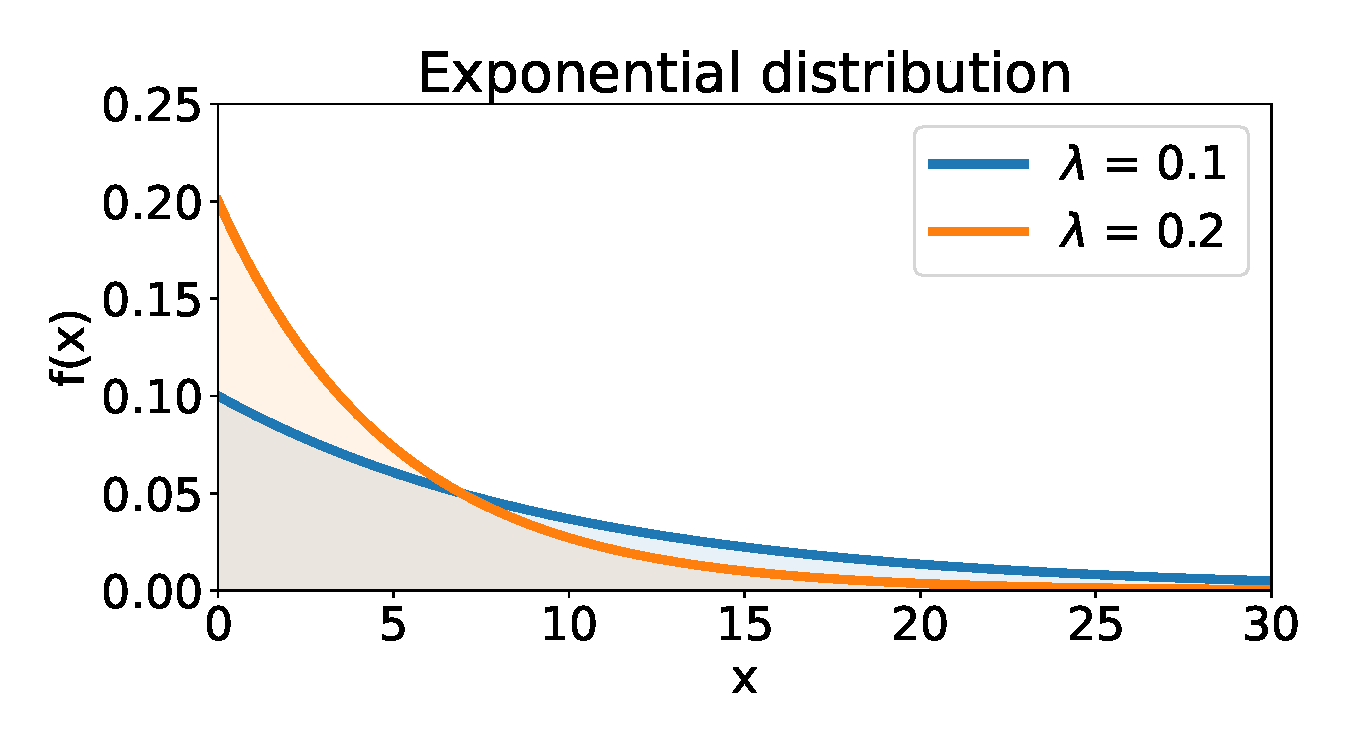
\includegraphics[width=.7\textwidth]{graphics/exponential_distribution.pdf}
    \end{center}$~$\\[-8ex]
    \begin{equation}
        \E[X] = \tfrac{1}{\lambda} \qquad \text{and} \qquad \V[X] = \tfrac{1}{\lambda^2}
    \end{equation}
\end{frame}
%%%%%%%%%%%%%%%%%%%%%%%%%%%%%%%%%%%%%%%%%%%%%%%%%%%%%%%%%%%%%%%%%%%%%%%%%%%%%%%%%%%%%%
%
%
%
%%%%%%%%%%%%%%%%%%%%%%%%%%%%%%%%%%%%%%%%%%%%%%%%%%%%%%%%%%%%%%%%%%%%%%%%%%%%%%%%%%%%%%
\begin{frame}{Exponential distribution}
    \begin{center}
        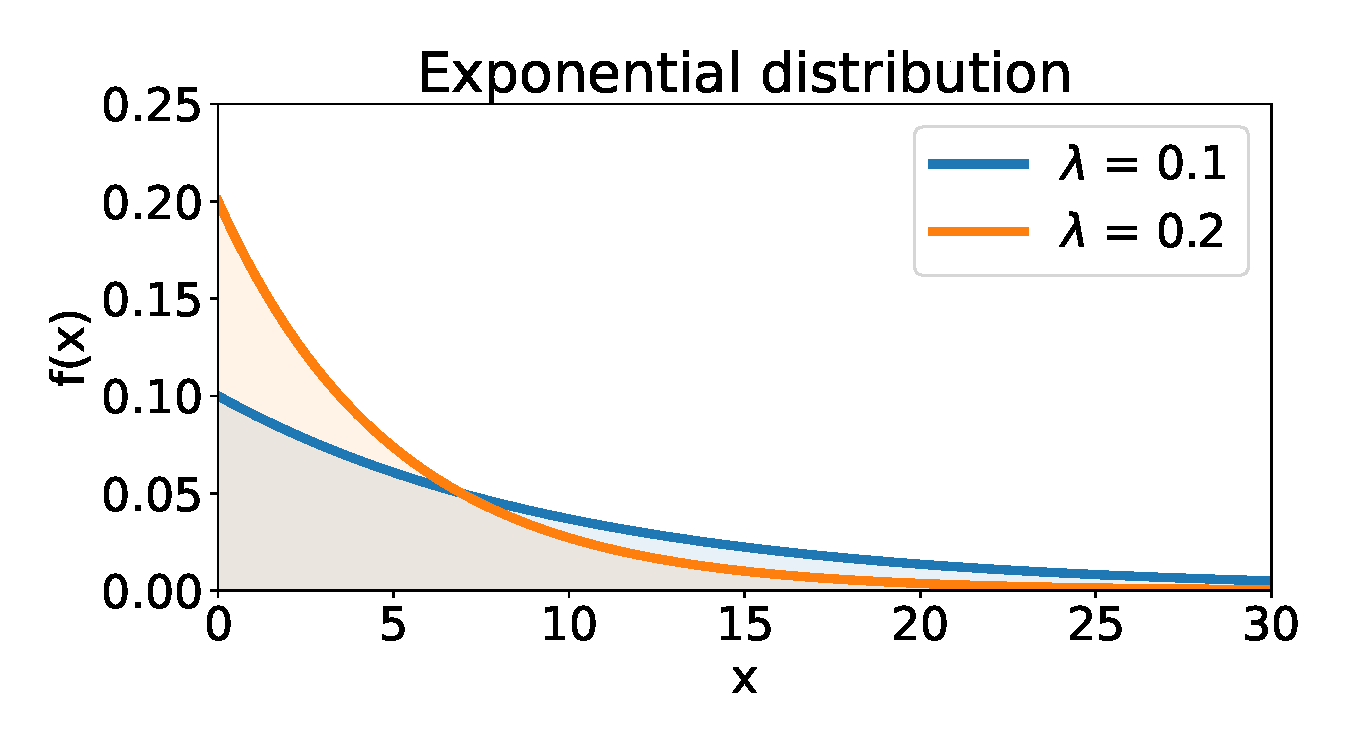
\includegraphics[width=.5\textwidth]{graphics/exponential_distribution.pdf}
    \end{center}
    \begin{block}{Example: Time until next mutation.}
        If mutations happen at rate $\theta$, then time to next mut. $\sim \text{Exp}(\theta)$.
    \end{block}
    \begin{itemize}
        \item Waiting time:
        \begin{itemize}
             \item Continuous time analog of geometric distribution.
         \end{itemize}
        \item Connection to poisson distribution:
        \begin{itemize}
            \item If mutations happen at rate $\theta$,
            \item then (\# mutations in time interval T) $\sim \text{Poi}(T \theta)$.
        \end{itemize}
    \end{itemize}
\end{frame}
%%%%%%%%%%%%%%%%%%%%%%%%%%%%%%%%%%%%%%%%%%%%%%%%%%%%%%%%%%%%%%%%%%%%%%%%%%%%%%%%%%%%%%
%
%
%
%%%%%%%%%%%%%%%%%%%%%%%%%%%%%%%%%%%%%%%%%%%%%%%%%%%%%%%%%%%%%%%%%%%%%%%%%%%%%%%%%%%%%%
\begin{frame}{Beta distribution}
    \begin{block}{Beta distribution}
        Flexible probability distribution for random values between 0 and 1.
    \end{block}
    \begin{columns}
        \begin{column}{.58\textwidth}
            \begin{itemize}
                \item Two parameters: $\alpha,\beta > 0$.
            \end{itemize}$~$\\[-4ex]
            \begin{equation}
                X \sim \text{Beta}(\alpha,\beta)
            \end{equation}$~$\\[-7ex]
            \begin{equation}
                f(x) = \tfrac{1}{B(\alpha,\beta)} x^{\alpha-1} (1-x)^{\beta-1}
            \end{equation}$~$\\[-5ex]
            \begin{equation}
                \E[X] = \tfrac{\alpha}{\alpha+\beta}
            \end{equation}$~$\\[-3ex]
            \begin{itemize}
                \item Useful as \textbf{prior} for probabilities~$p$, since $p \in [0,1]$.
                \item Conjugate prior for binomial distribution.
                \item Stationary distribution for some Wright-Fisher models.
            \end{itemize}
        \end{column}
        \begin{column}{.42\textwidth}
            \begin{center}
                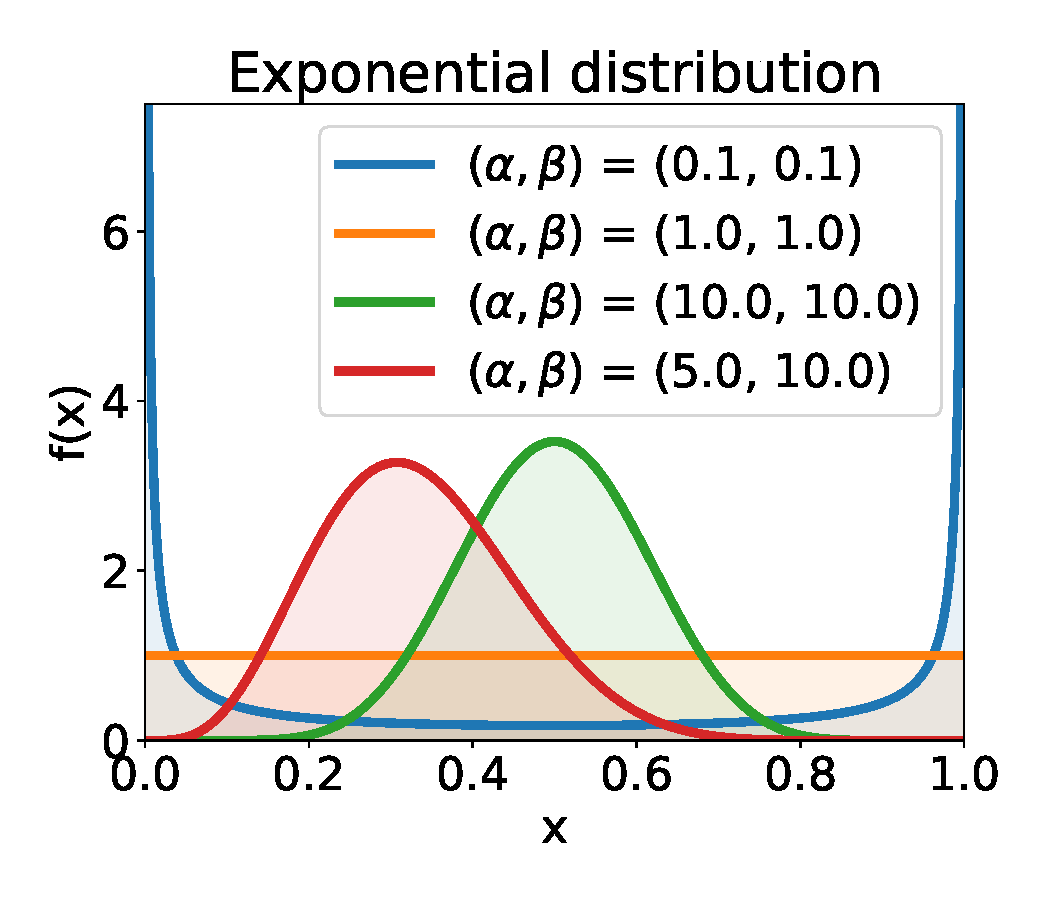
\includegraphics[width=\textwidth]{graphics/beta_distribution.pdf}
            \end{center}
        \end{column}
    \end{columns}
\end{frame}
%%%%%%%%%%%%%%%%%%%%%%%%%%%%%%%%%%%%%%%%%%%%%%%%%%%%%%%%%%%%%%%%%%%%%%%%%%%%%%%%%%%%%%
%
%
%
%%%%%%%%%%%%%%%%%%%%%%%%%%%%%%%%%%%%%%%%%%%%%%%%%%%%%%%%%%%%%%%%%%%%%%%%%%%%%%%%%%%%%%
\begin{frame}
    \begin{center}
        {\Large 5 minute intermission.}
    \end{center}
\end{frame}
%%%%%%%%%%%%%%%%%%%%%%%%%%%%%%%%%%%%%%%%%%%%%%%%%%%%%%%%%%%%%%%%%%%%%%%%%%%%%%%%%%%%%%
%
%
%
%%%%%%%%%%%%%%%%%%%%%%%%%%%%%%%%%%%%%%%%%%%%%%%%%%%%%%%%%%%%%%%%%%%%%%%%%%%%%%%%%%%%%%
\begin{frame}{Population genomic simulations}
    Some popular tools:
    \begin{itemize}
        \item \texttt{SLiM} (5.0\textit{; Haller, Ralph, Messer; 2025}).
        \begin{itemize}
            \item Forward-in-time.
            \item Very flexible; models various forms of selection.
            \item Simulates whole genomes for entire population.
        \end{itemize}
        \item \texttt{msprime} (\textit{Baumdicker et al.; 2021}).
        \begin{itemize}
            \item Backward-in-time (coalescent).
            \item Efficient for large scale neutral simulations.
            \item Simulates whole genomes for a population sample.
        \end{itemize}
    \end{itemize}
    \begin{block}{}
        \begin{itemize}
            \item All build on these elementary distributions.
            \item Combine distributions in the right way with the right parameters to model complex population genetic processes.
        \end{itemize}
    \end{block}
\end{frame}
%%%%%%%%%%%%%%%%%%%%%%%%%%%%%%%%%%%%%%%%%%%%%%%%%%%%%%%%%%%%%%%%%%%%%%%%%%%%%%%%%%%%%%
%
%
%
%%%%%%%%%%%%%%%%%%%%%%%%%%%%%%%%%%%%%%%%%%%%%%%%%%%%%%%%%%%%%%%%%%%%%%%%%%%%%%%%%%%%%%
\begin{frame}{(Summary) statistics}
    Compute summary of genomic data.
    \begin{itemize}
        \item Or multiple summaries.
    \end{itemize}
    \begin{block}{}
        Certain summary (statistics) informative about certain processes:
    \end{block}
    \begin{itemize}
        \item Pairwise diversity $\pi$:
        \begin{itemize}
            \item Mutation rate, effective population size.
        \end{itemize}
        \item $\text{F}_\text{ST}$, F-statistics:
        \begin{itemize}
            \item Population structure, selection.
        \end{itemize}
        \item Tajima's D:
        \begin{itemize}
            \item Neutrality, selection, effective population size.
        \end{itemize}
        \item Site-Frequency-Spectrum (SFS):
        \begin{itemize}
            \item Demography, selection, ...
        \end{itemize}
        \item ...
    \end{itemize}
\end{frame}
%%%%%%%%%%%%%%%%%%%%%%%%%%%%%%%%%%%%%%%%%%%%%%%%%%%%%%%%%%%%%%%%%%%%%%%%%%%%%%%%%%%%%%
%
%
%
%%%%%%%%%%%%%%%%%%%%%%%%%%%%%%%%%%%%%%%%%%%%%%%%%%%%%%%%%%%%%%%%%%%%%%%%%%%%%%%%%%%%%%
\begin{frame}{Likelihood-based inference of model parameters}
    Given:
    \begin{itemize}
        \item Observed data $D$:
        \begin{itemize}
            \item Genomic sequences of sampled individuals.
            \item Alleles of sampled individuals at specific locus.
            \item ...
        \end{itemize}
        \item Model for data $D$ that has parameters $\Theta = (\theta_1, \ldots, \theta_n)$:
        \begin{itemize}
            \item Demographic parameters.
            \item Recombination rates.
            \item Selection coefficients.
            \item ...
        \end{itemize}
    \end{itemize}
    Can define
    \begin{block}{Likelihood: Probability of data given parameter.}
        \begin{equation}
            L(\Theta) := \P_\Theta\{D\}
        \end{equation}
    \end{block}
    If $L(\Theta_1) > L(\Theta_2)$, then data $D$ more likely under parameters $\Theta_1$.
    \begin{itemize}
        \item Parameters $\Theta_1$ explain data better.
    \end{itemize}
\end{frame}
%%%%%%%%%%%%%%%%%%%%%%%%%%%%%%%%%%%%%%%%%%%%%%%%%%%%%%%%%%%%%%%%%%%%%%%%%%%%%%%%%%%%%%
%
%
%
%%%%%%%%%%%%%%%%%%%%%%%%%%%%%%%%%%%%%%%%%%%%%%%%%%%%%%%%%%%%%%%%%%%%%%%%%%%%%%%%%%%%%%
\begin{frame}{Maximum likelihood}
    \begin{block}{Maximum likelihood estimate}
        Find the parameter $\Theta^*$ that maximize the likelihood $L(\Theta)$.
    \end{block}
    \begin{itemize}
        \item These parameters explain data $D$ best under given model.
        \item Equivalently: Maximize log-likelihood: $\log L(\Theta)$.
    \end{itemize}
    \begin{center}
        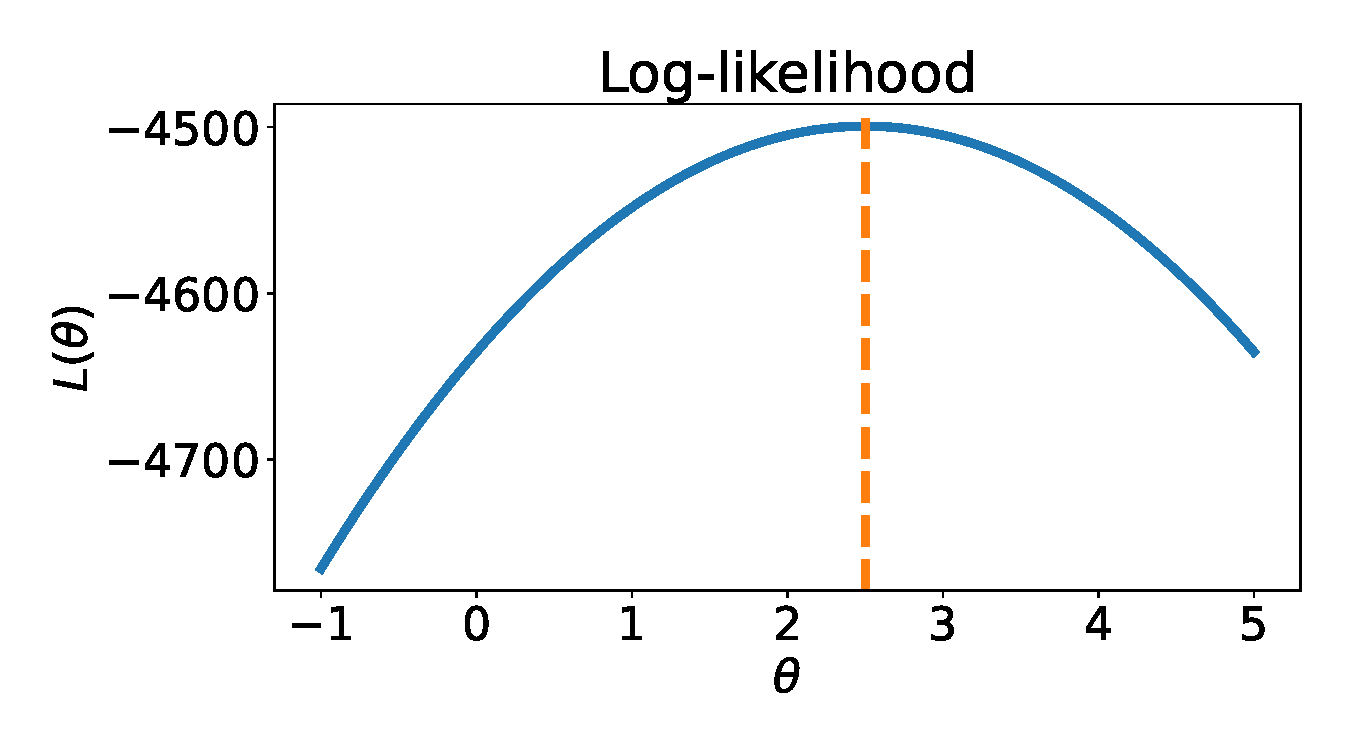
\includegraphics[width=.6\textwidth]{graphics/log_likelihood.pdf}
    \end{center}$~$\\[-6ex]
    \begin{block}{}
        \begin{itemize}
            \item Many methods throughout the course infer model parameters from genomic data using this approach.
        \end{itemize}
    \end{block}
\end{frame}
%%%%%%%%%%%%%%%%%%%%%%%%%%%%%%%%%%%%%%%%%%%%%%%%%%%%%%%%%%%%%%%%%%%%%%%%%%%%%%%%%%%%%%
%
%
%
%%%%%%%%%%%%%%%%%%%%%%%%%%%%%%%%%%%%%%%%%%%%%%%%%%%%%%%%%%%%%%%%%%%%%%%%%%%%%%%%%%%%%%
\begin{frame}
    Next:
    \begin{block}{}
        Bayesian inference.
    \end{block}
    But for that we need:
    \begin{itemize}
        \item Conditional probability.
        \item Bayes' theorem.
    \end{itemize}
\end{frame}
%%%%%%%%%%%%%%%%%%%%%%%%%%%%%%%%%%%%%%%%%%%%%%%%%%%%%%%%%%%%%%%%%%%%%%%%%%%%%%%%%%%%%%
%
%
%
%%%%%%%%%%%%%%%%%%%%%%%%%%%%%%%%%%%%%%%%%%%%%%%%%%%%%%%%%%%%%%%%%%%%%%%%%%%%%%%%%%%%%%
\begin{frame}{Conditional probability}
    \begin{block}{}
        Probability of specific outcome given information about outcome.
    \end{block}
    Example: $X \sim \text{Bin}(20,0.4)$, \textbf{conditioned} on $X \geq 8$.
    \begin{block}{}
        \begin{equation}
            \P\{X = k | X \geq 8\} := \frac{\alert<2>{\P\{X = k , X \geq 8\}}}{\alert<3>{\P\{X \geq 8\}}}
        \end{equation}
    \end{block}
    \begin{itemize}
        \item \alert<2>{Restrict distribution}, and \alert<3>{re-normalize} (sum to 1).
    \end{itemize}
    \begin{center}
\only<1>{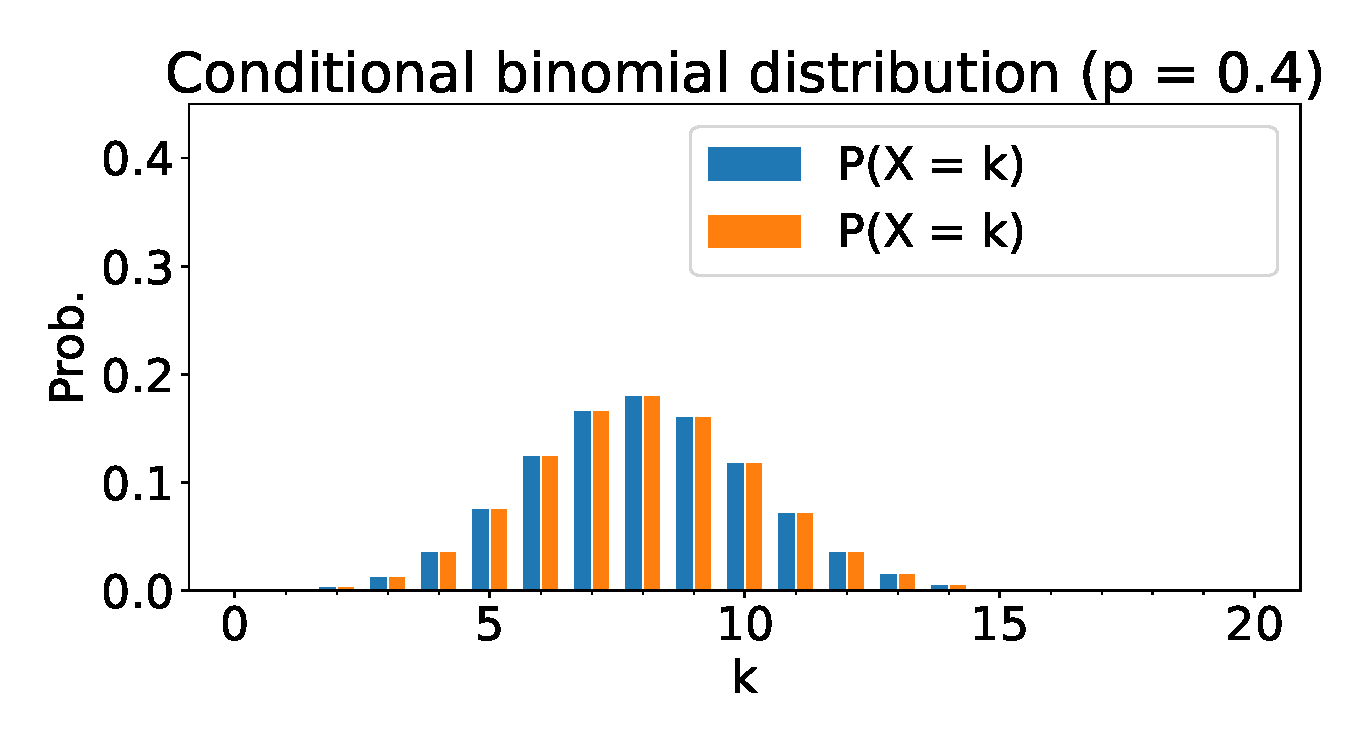
\includegraphics[width=.7\textwidth]{graphics/conditional_binomial_uncond.pdf}}%
\only<2>{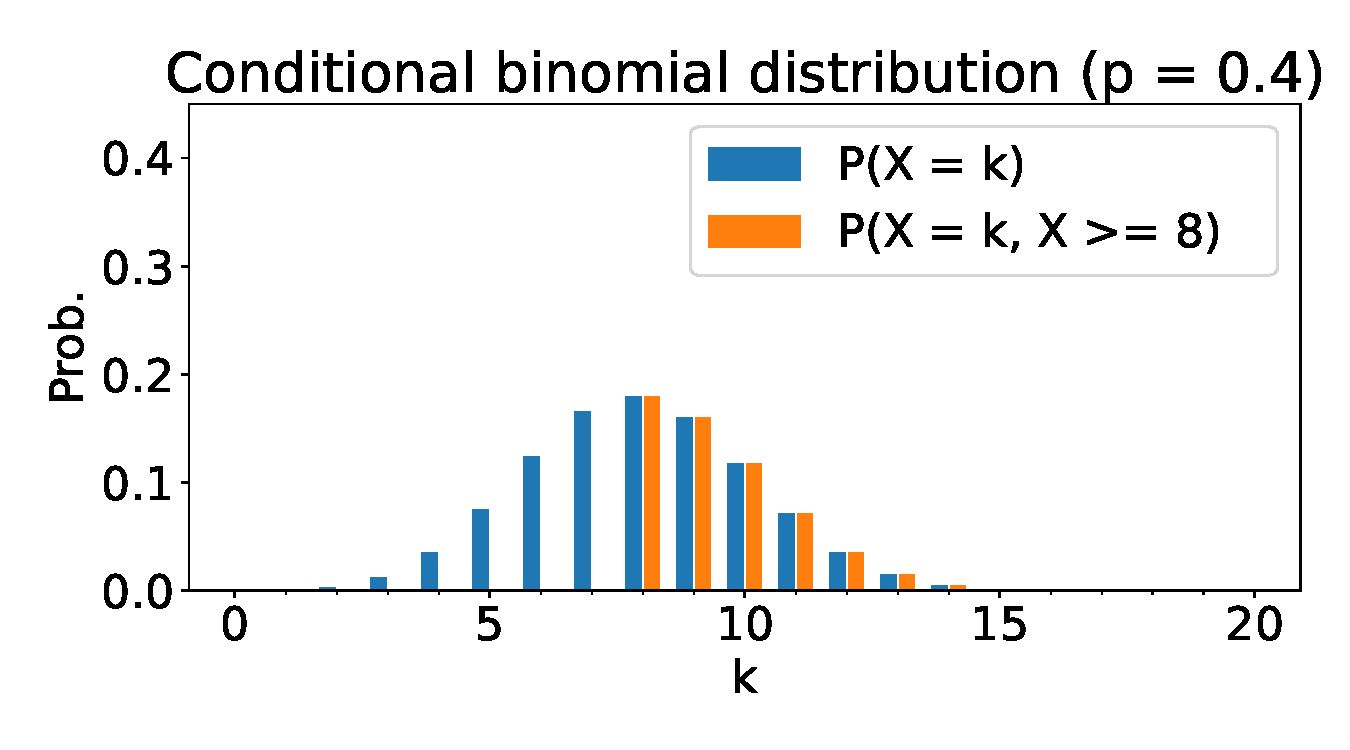
\includegraphics[width=.7\textwidth]{graphics/conditional_binomial_restrict.pdf}}%
\only<3,4>{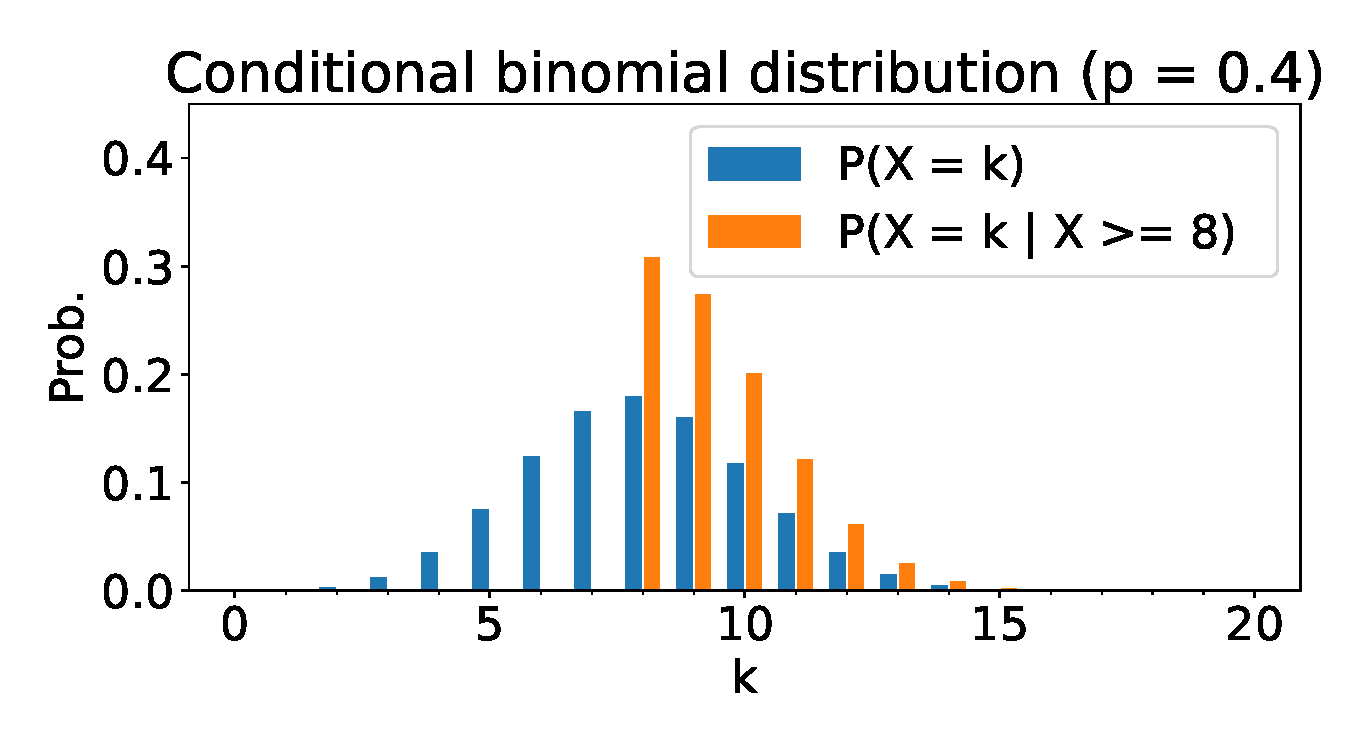
\includegraphics[width=.7\textwidth]{graphics/conditional_binomial_cond.pdf}}%
    \end{center}
\end{frame}
%%%%%%%%%%%%%%%%%%%%%%%%%%%%%%%%%%%%%%%%%%%%%%%%%%%%%%%%%%%%%%%%%%%%%%%%%%%%%%%%%%%%%%
%
%
%
%%%%%%%%%%%%%%%%%%%%%%%%%%%%%%%%%%%%%%%%%%%%%%%%%%%%%%%%%%%%%%%%%%%%%%%%%%%%%%%%%%%%%%
\begin{frame}{Conditional probability}
    In general:
    \begin{itemize}
        \item Probability of outcome $A$.
        \item Conditioned on $B$.
    \end{itemize}
    \begin{block}{Conditional probability}
        \begin{equation}
            \P\{A|B\} := \frac{\P\{A,B\}}{\P\{B\}}
        \end{equation}
    \end{block}
    Immediately yields Bayes' theorem:
    \begin{block}{Bayes' theorem}
        \begin{equation}
            \P\{A|B\} = \frac{\P\{B|A\}\P\{A\}}{\P\{B\}}
        \end{equation}        
    \end{block}
    \begin{itemize}
        \item Can compute conditional $\P\{A|B\}$ in terms of $\P\{B|A\}$.
    \end{itemize}
\end{frame}
%%%%%%%%%%%%%%%%%%%%%%%%%%%%%%%%%%%%%%%%%%%%%%%%%%%%%%%%%%%%%%%%%%%%%%%%%%%%%%%%%%%%%%
%
%
%
%%%%%%%%%%%%%%%%%%%%%%%%%%%%%%%%%%%%%%%%%%%%%%%%%%%%%%%%%%%%%%%%%%%%%%%%%%%%%%%%%%%%%%
\begin{frame}{Bayesian inference}
    Interpret:
    \begin{itemize}
        \item $A$ as model parameter $\Theta$.
        \item $B$ as data $D$.
    \end{itemize}
    Then:
    \begin{block}{}
        \begin{equation}
            \P \{ \text{parameter }\Theta | \text{data }D \} = \frac{\P \{ \text{data }D | \text{parameter }\Theta \} \P \{\text{parameter }\Theta\}}{\P \{\text{data }D\}}
        \end{equation}
    \end{block}
    With:
    \begin{itemize}
        \item \textbf{Prior}: $\P \{\text{parameter }\Theta\}$
        \item \textbf{Likelihood}: $\P \{ \text{data }D | \text{parameter }\Theta \}$
        \item \textbf{Posterior}: $\P \{ \text{parameter }\Theta | \text{data }D \}$
    \end{itemize}
\end{frame}
%%%%%%%%%%%%%%%%%%%%%%%%%%%%%%%%%%%%%%%%%%%%%%%%%%%%%%%%%%%%%%%%%%%%%%%%%%%%%%%%%%%%%%
%
%
%
%%%%%%%%%%%%%%%%%%%%%%%%%%%%%%%%%%%%%%%%%%%%%%%%%%%%%%%%%%%%%%%%%%%%%%%%%%%%%%%%%%%%%%
\begin{frame}{Bayesian inference}
    \begin{block}{}
        \begin{equation}
            \P \{ \text{parameter }\Theta | \text{data }D \} = \frac{\P \{ \text{data }D | \text{parameter }\Theta \} \P \{\text{parameter }\Theta\}}{\P \{\text{data }D\}}
        \end{equation}
    \end{block}
    \begin{center}
\only<1>{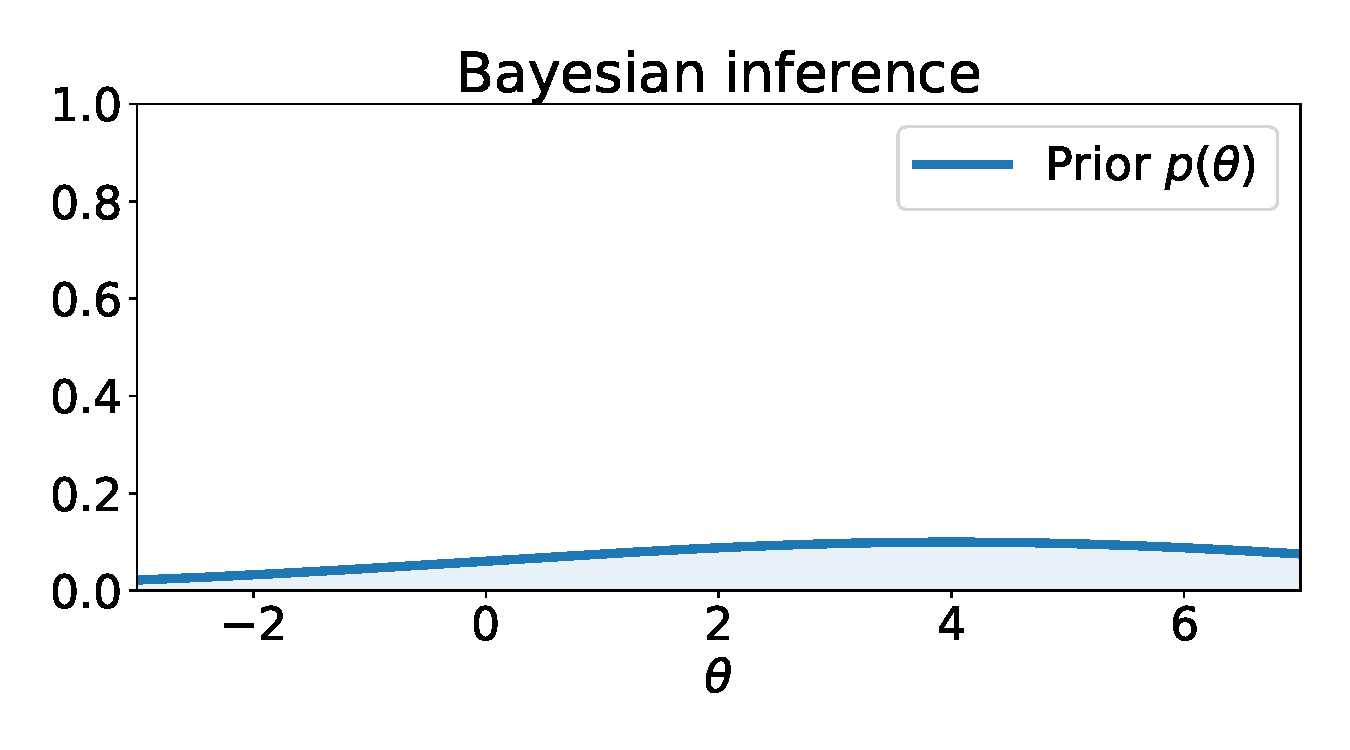
\includegraphics[width=.7\textwidth]{graphics/bayesian_prior.pdf}}%
\only<2>{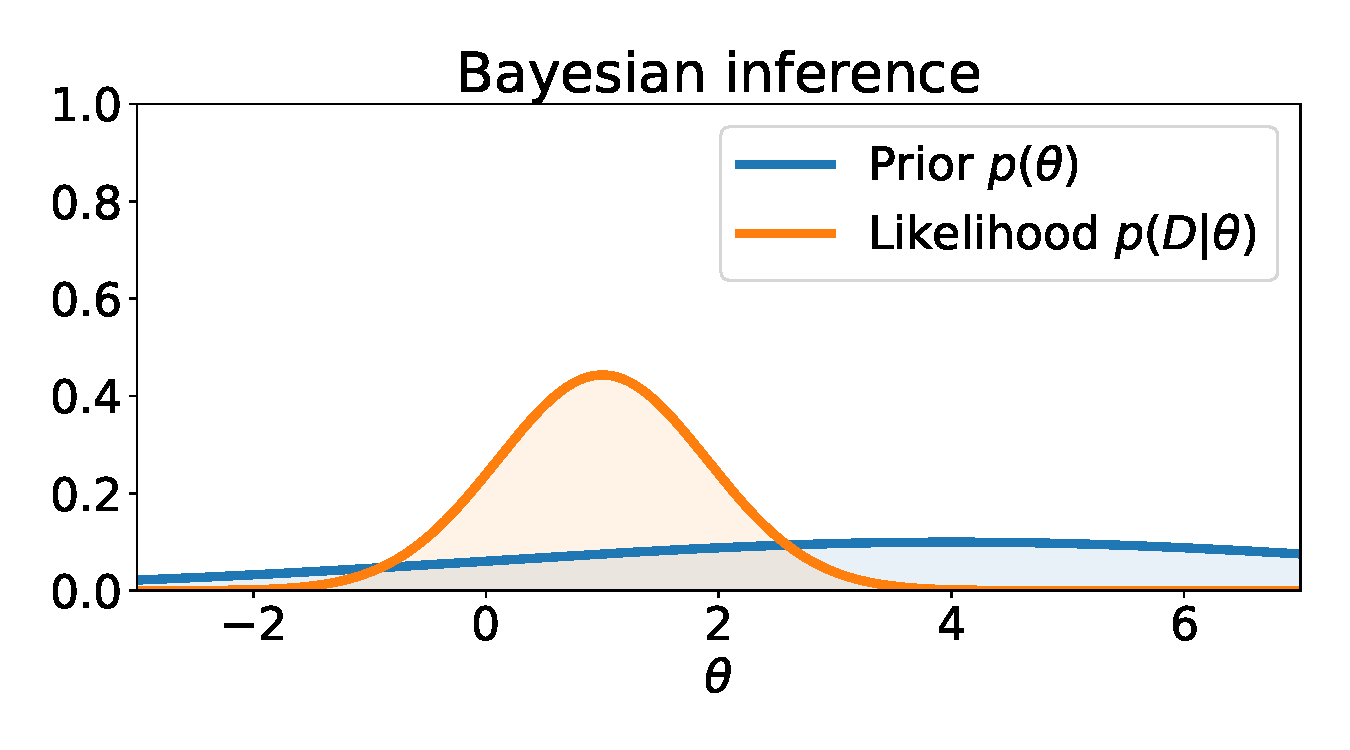
\includegraphics[width=.7\textwidth]{graphics/bayesian_likelihood.pdf}}%
\only<3->{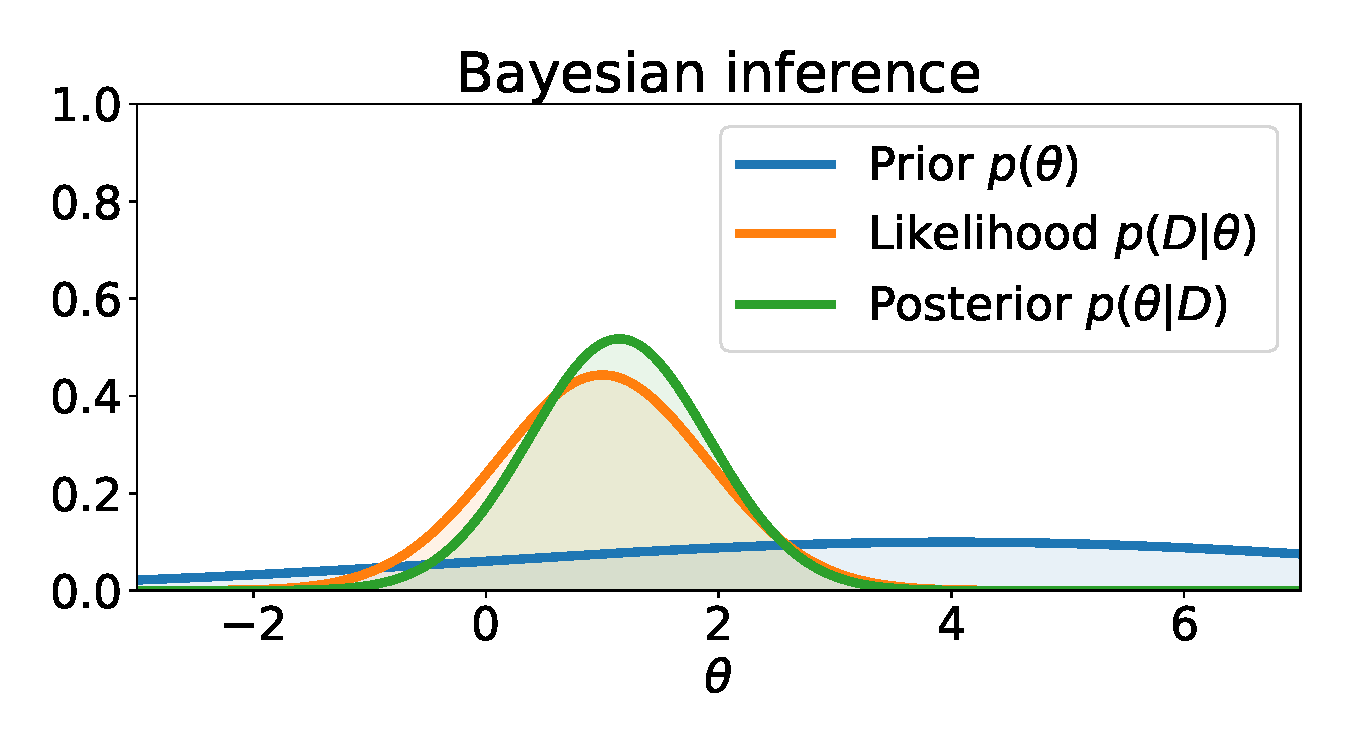
\includegraphics[width=.7\textwidth]{graphics/bayesian_posterior.pdf}}%
    \end{center}
\end{frame}
%%%%%%%%%%%%%%%%%%%%%%%%%%%%%%%%%%%%%%%%%%%%%%%%%%%%%%%%%%%%%%%%%%%%%%%%%%%%%%%%%%%%%%
%
%
%
%%%%%%%%%%%%%%%%%%%%%%%%%%%%%%%%%%%%%%%%%%%%%%%%%%%%%%%%%%%%%%%%%%%%%%%%%%%%%%%%%%%%%%
\begin{frame}{Bayesian inference}
    \begin{block}{}
        \begin{equation}
            \P \{ \text{parameter }\Theta | \text{data }D \} = \frac{\P \{ \text{data }D | \text{parameter }\Theta \} \P \{\text{parameter }\Theta\}}{\P \{\text{data }D\}}
        \end{equation}
    \end{block}
    \begin{itemize}
        \item Can sometimes be solved analytically.
        \begin{itemize}
            \item Exact formula for posterior distribution.
        \end{itemize}
        \item Often analytic solution not possible.
        \begin{itemize}
            \item Sample from posterior distribution.
            \item Monte-Carlo Markov Chain (MCMC).
            \item Approximate Bayesian Computation (ABC).
        \end{itemize}
        \item More details in dedicated lectures.
    \end{itemize}
\end{frame}
%%%%%%%%%%%%%%%%%%%%%%%%%%%%%%%%%%%%%%%%%%%%%%%%%%%%%%%%%%%%%%%%%%%%%%%%%%%%%%%%%%%%%%
%
%
%
%%%%%%%%%%%%%%%%%%%%%%%%%%%%%%%%%%%%%%%%%%%%%%%%%%%%%%%%%%%%%%%%%%%%%%%%%%%%%%%%%%%%%%
\begin{frame}{Latent variables}
    \begin{block}{Latent variable}
        Random outcome depends on other random outcome.
    \end{block}
    Example: \# mutations sample $i$ and $j$ differ in certain genomic region (of length $L$ bp).
    \begin{itemize}
        \item Per gener.\ per bp mutation rate $u$.
        \item If most recent common ancestor of $i$ and $j$ at $T$ gener.\ ago.
        \item Then $i$ and $j$ separated by $2T$ generations.
        \item \# mut. $i$ and $j$ differ is $\sim \text{Poi}(2T \cdot u \cdot L)$.
        \item But $T$ random, $T \sim \text{Exp}(\tfrac{1}{2N})$. 
    \end{itemize}
    \begin{block}{}
        \begin{equation}
            \begin{split}
                \P\{\pi_{i,j} = k\} & = \int_0^\infty \P\{\pi_{i,j} = k | T\} \P\{T\} dT\\
                    & = \int_0^\infty \tfrac{(2T \cdot u \cdot L)^k e^{-k}}{k!} \tfrac{1}{2N} \exp(-\tfrac{1}{2N}T) dT
            \end{split}
        \end{equation}
    \end{block}
\end{frame}
%%%%%%%%%%%%%%%%%%%%%%%%%%%%%%%%%%%%%%%%%%%%%%%%%%%%%%%%%%%%%%%%%%%%%%%%%%%%%%%%%%%%%%
%
%
%
%%%%%%%%%%%%%%%%%%%%%%%%%%%%%%%%%%%%%%%%%%%%%%%%%%%%%%%%%%%%%%%%%%%%%%%%%%%%%%%%%%%%%%
\begin{frame}{Optimization and gradient descent}
    \begin{block}{Task}
        Find parameters $\Theta$ that maximize/minimize function $L(\Theta)$.
    \end{block}
    \begin{itemize}
        \item Maximum-likelihood:
        \begin{itemize}
            \item Likelihood $L(\Theta)$: How likely observed data for given $\Theta$.
            \item Find parameters $\Theta^*$ that yield highest likelihood.
            \item Explain data best.
        \end{itemize}
        \item Machine learning:
        \begin{itemize}
            \item Artificial neural networks (ANNs) have many parameters $\Theta$.
            \begin{itemize}
                \item Chat-GTP 3.5: 175 billion parameters.
            \end{itemize}
            \item Loss function $L(\Theta)$ captures how well ANN performs tasks.
            \item Find parameters $\Theta^*$ that minimize loss.
            \item Performs best on the given tasks.
        \end{itemize}
    \end{itemize}
    \begin{block}{}
        Often not possible to find global optimum.
        \begin{itemize}
            \item Find $\Theta$ were $L(\Theta)$ as large/small as possible.
        \end{itemize}
    \end{block}
    Maximizing is just minimizing with opposite sign.
\end{frame}
%%%%%%%%%%%%%%%%%%%%%%%%%%%%%%%%%%%%%%%%%%%%%%%%%%%%%%%%%%%%%%%%%%%%%%%%%%%%%%%%%%%%%%
%
%
%
%%%%%%%%%%%%%%%%%%%%%%%%%%%%%%%%%%%%%%%%%%%%%%%%%%%%%%%%%%%%%%%%%%%%%%%%%%%%%%%%%%%%%%
\begin{frame}{Optimization and gradient descent}
    Minimize $L(\theta)$:
    \begin{block}{Derivative/gradient}
        Take derivative of $L(\theta)$ with respect to $\theta$: $\tfrac{d}{d\theta}L(\theta)$.
        \begin{itemize}
            \item If $\tfrac{d}{d\theta}L(\theta) > 0$, then $\theta \leftarrow$ yields $L(\theta) \downarrow$.
            \item If $\tfrac{d}{d\theta}L(\theta) < 0$, then $\theta \rightarrow$ yields $L(\theta) \downarrow$.
        \end{itemize}
    \end{block}
    \begin{columns}
        \begin{column}{.6\textwidth}
            At minimum $\theta^*$:
            \begin{itemize}
                \item Neither $\theta \leftarrow$ nor $\theta \rightarrow$ yields $L(\theta) \downarrow$.
                \item Thus, $\tfrac{d}{d\theta}L(\theta^*) = 0$.
            \end{itemize}
            \begin{block}{}
                In some applications, possible to find $\theta^*$ by solving $\tfrac{d}{d\theta}L(\theta^*) = 0$ analytically.
            \end{block}
        \end{column}
        \begin{column}{.4\textwidth}
\only<1>{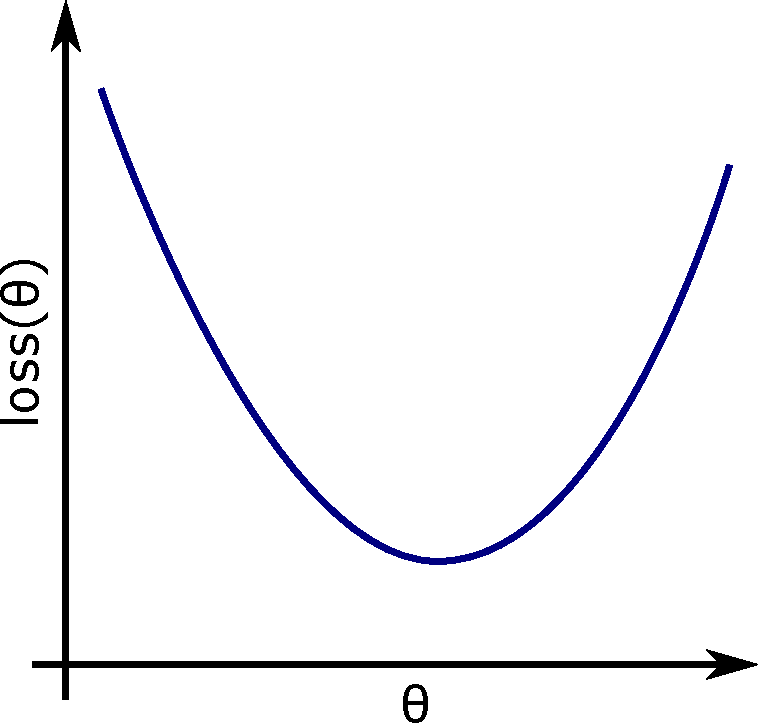
\includegraphics[width=\textwidth]{graphics/gradient_descent_blank.pdf}}%
\only<2>{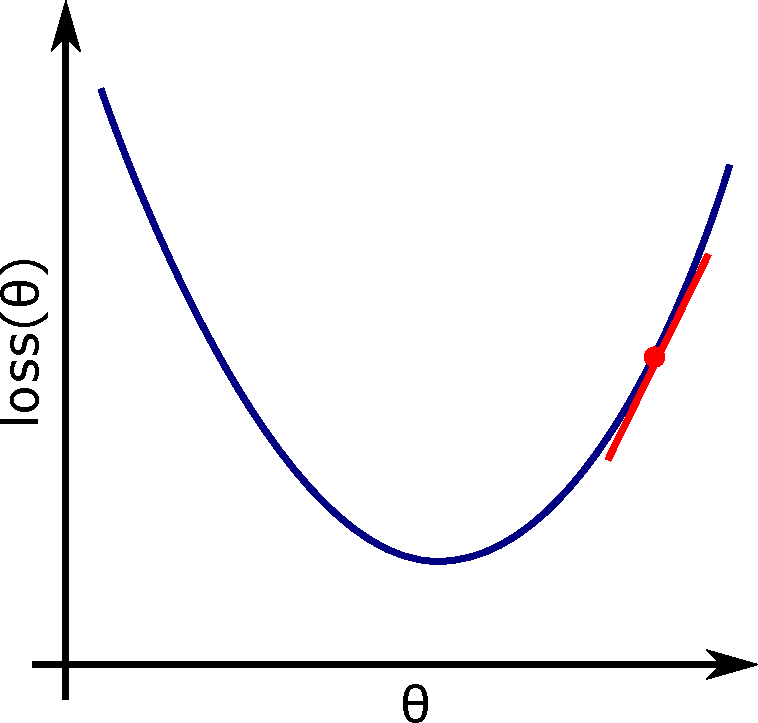
\includegraphics[width=\textwidth]{graphics/gradient_descent_pos_one.pdf}}%
\only<3>{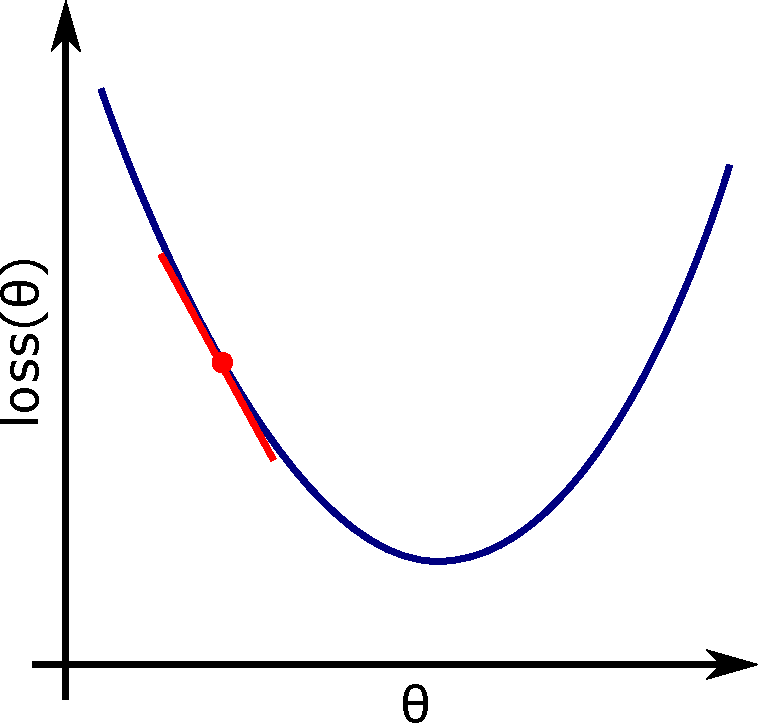
\includegraphics[width=\textwidth]{graphics/gradient_descent_neg_one.pdf}}%
\only<4->{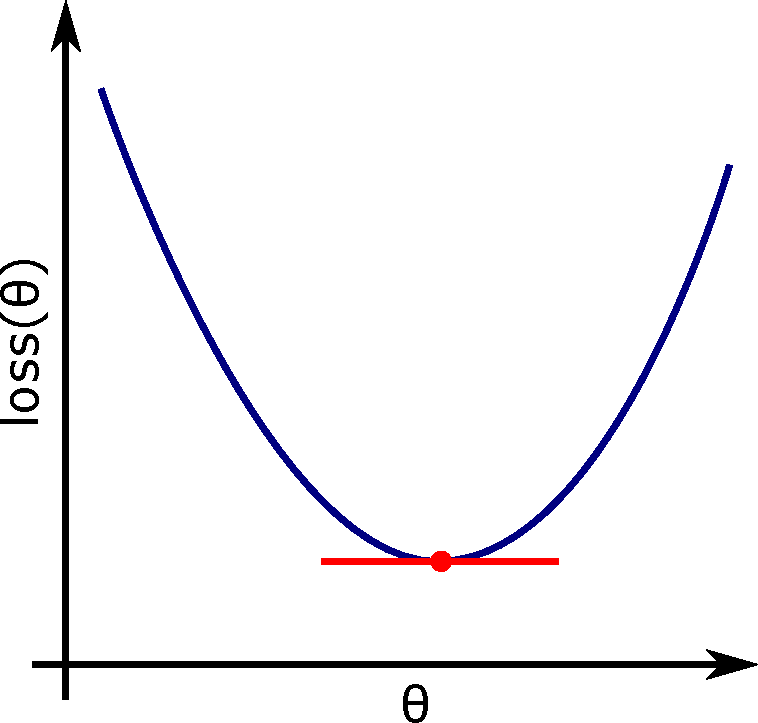
\includegraphics[width=\textwidth]{graphics/gradient_descent_opt.pdf}}%
        \end{column}
    \end{columns}
\end{frame}
%%%%%%%%%%%%%%%%%%%%%%%%%%%%%%%%%%%%%%%%%%%%%%%%%%%%%%%%%%%%%%%%%%%%%%%%%%%%%%%%%%%%%%
%
%
%
%%%%%%%%%%%%%%%%%%%%%%%%%%%%%%%%%%%%%%%%%%%%%%%%%%%%%%%%%%%%%%%%%%%%%%%%%%%%%%%%%%%%%%
\begin{frame}{Optimization and gradient descent}
    If not possible to solve $\tfrac{d}{d\theta}L(\theta^*) = 0$, then optimize $\theta$ stepwise.\\
    \begin{columns}
        \begin{column}{.6\textwidth}
            \begin{block}{Gradient descent}
                \begin{itemize}
                    \item Start at $\theta^{(0)}$.
                    \item Update $\theta^{(k)} \to \theta^{(k+1)}$:
                    \begin{itemize}
                        \item If $\tfrac{d}{d\theta}L(\theta^{(k)}) < 0$, then $\theta^{(k)} \rightarrow$.
                        \item If $\tfrac{d}{d\theta}L(\theta^{(k)}) > 0$, then $\theta^{(k)} \leftarrow$.
                    \end{itemize}
                    \item Until stopping criterion reached.
                \end{itemize}
            \end{block}
        \end{column}
        \begin{column}{.4\textwidth}
            \begin{center}
\only<1>{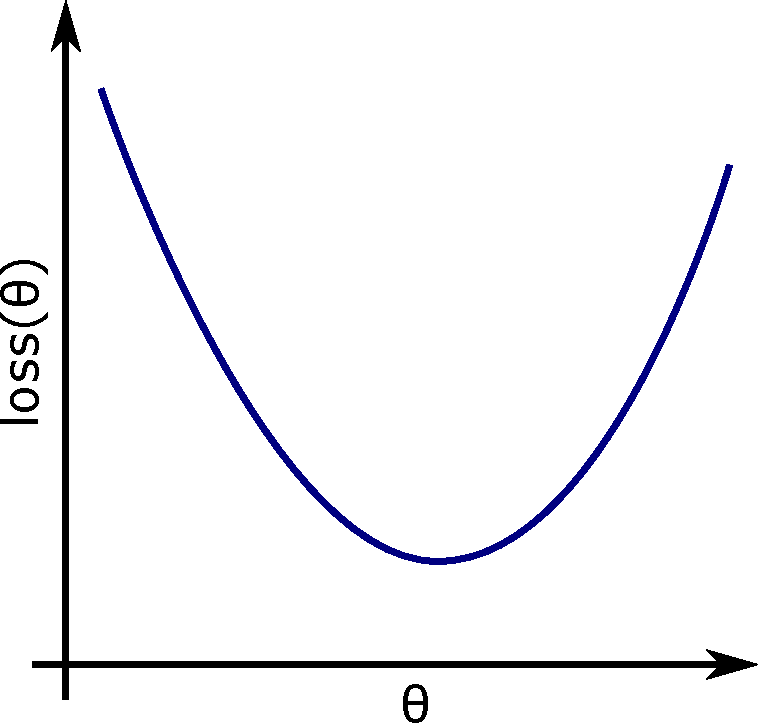
\includegraphics[width=\textwidth]{graphics/gradient_descent_blank.pdf}}%
\only<2>{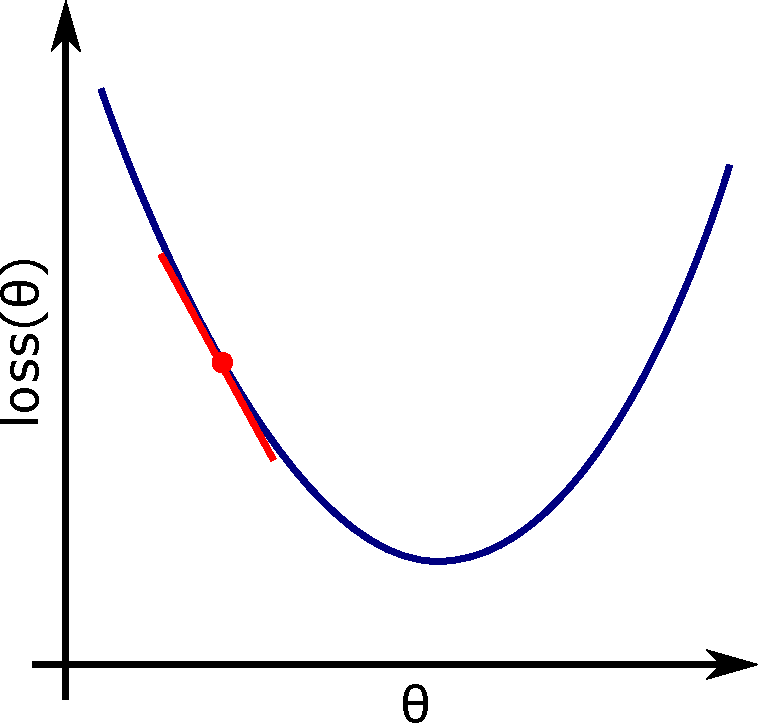
\includegraphics[width=\textwidth]{graphics/gradient_descent_neg_one.pdf}}%
\only<3>{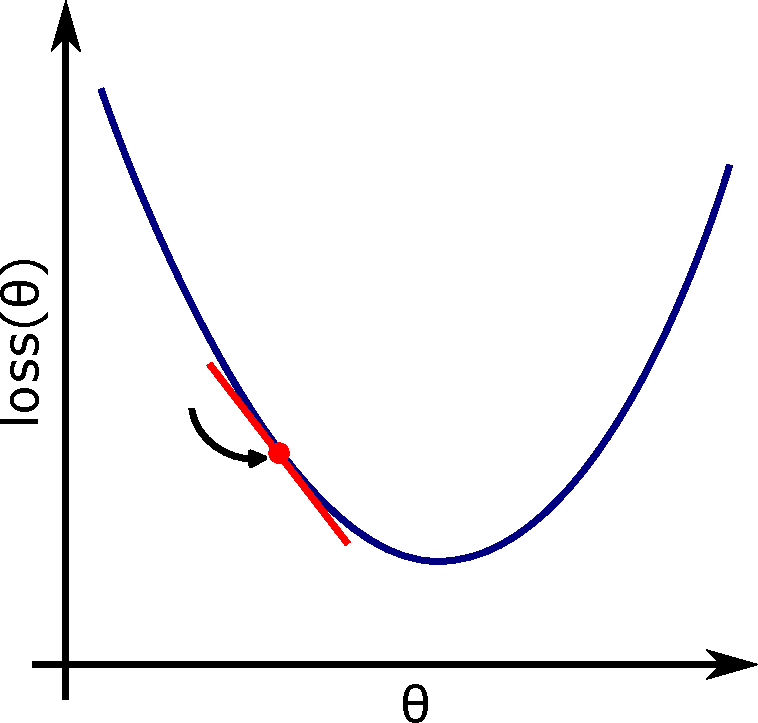
\includegraphics[width=\textwidth]{graphics/gradient_descent_neg_two.pdf}}%
\only<4->{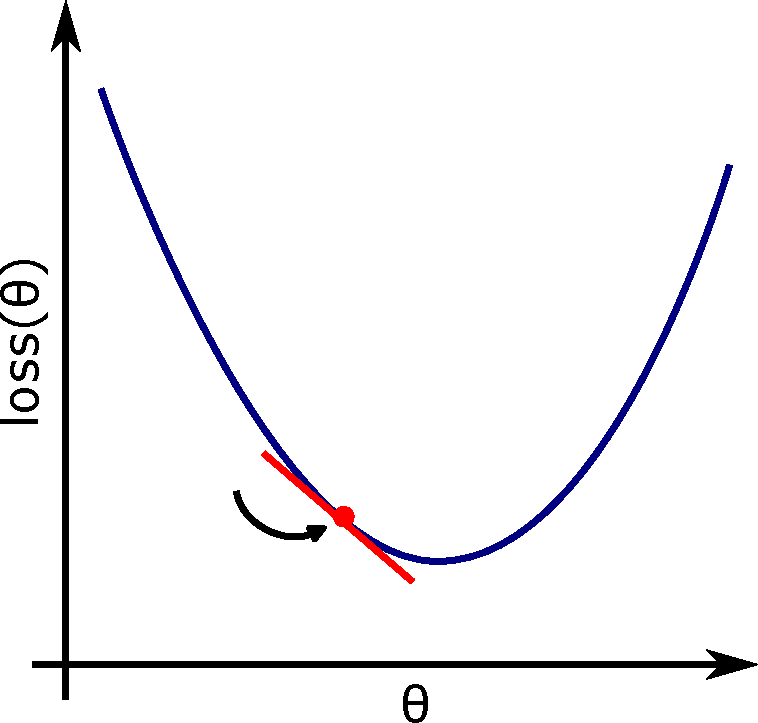
\includegraphics[width=\textwidth]{graphics/gradient_descent_neg_three.pdf}}%
            \end{center}
        \end{column}
    \end{columns}
    \begin{itemize}
        \item Many maximum-likelihood methods in population genomics use version of this strategy.
        \item Almost all training of ANNs uses versions of this.
    \end{itemize}
\end{frame}
%%%%%%%%%%%%%%%%%%%%%%%%%%%%%%%%%%%%%%%%%%%%%%%%%%%%%%%%%%%%%%%%%%%%%%%%%%%%%%%%%%%%%%
%
%
%
%%%%%%%%%%%%%%%%%%%%%%%%%%%%%%%%%%%%%%%%%%%%%%%%%%%%%%%%%%%%%%%%%%%%%%%%%%%%%%%%%%%%%%
\begin{frame}{Optimization and gradient descent}
    If more than one parameter:
    \begin{itemize}
        \item Gradient descent in multiple dimensions:
    \end{itemize}
    \begin{center}
        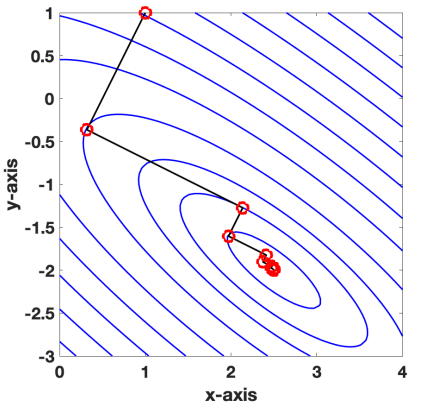
\includegraphics[width=.5\textwidth]{graphics/Steepest_descent_convergence_path_for_A_=_2_2,_2_3.png}\\\tiny{\url{https://en.wikipedia.org/wiki/Gradient\_descent}}
    \end{center}
\end{frame}
%%%%%%%%%%%%%%%%%%%%%%%%%%%%%%%%%%%%%%%%%%%%%%%%%%%%%%%%%%%%%%%%%%%%%%%%%%%%%%%%%%%%%%
%
%
%
%%%%%%%%%%%%%%%%%%%%%%%%%%%%%%%%%%%%%%%%%%%%%%%%%%%%%%%%%%%%%%%%%%%%%%%%%%%%%%%%%%%%%%
\begin{frame}
    \begin{center}
        That's it for today. Enjoy the course next week!
    \end{center}
\end{frame}
%%%%%%%%%%%%%%%%%%%%%%%%%%%%%%%%%%%%%%%%%%%%%%%%%%%%%%%%%%%%%%%%%%%%%%%%%%%%%%%%%%%%%%
%
%
%
%%%%%%%%%%%%%%%%%%%%%%%%%%%%%%%%%%%%%%%%%%%%%%%%%%%%%%%%%%%%%%%%%%%%%%%%%%%%%%%%%%%%%%
\end{document}
